%definira klasu dokumenta 
\documentclass[12pt]{report} 

%prostor izmedu naredbi \documentclass i \begin{document} se zove uvod. U njemu se nalaze naredbe koje se odnose na cijeli dokument

%osnovni LaTex ne može riješiti sve probleme, pa se koriste različiti paketi koji olakšavaju izradu željenog dokumenta
\usepackage[croatian]{babel} 
\usepackage{amssymb}
\usepackage{amsmath}
\usepackage{txfonts}
\usepackage{mathdots}
\usepackage{titlesec}
\usepackage{array}
\usepackage{lastpage}
\usepackage{etoolbox}
\usepackage{tabularray}
\usepackage{color, colortbl}
\usepackage{adjustbox}
\usepackage{geometry}
\usepackage[classicReIm]{kpfonts}
\usepackage{hyperref}
\usepackage{fancyhdr}

\usepackage{float}
\usepackage{setspace}
\restylefloat{table}


\patchcmd{\chapter}{\thispagestyle{plain}}{\thispagestyle{fancy}}{}{} %redefiniranje stila stranice u paketu fancyhdr

%oblik naslova poglavlja
\titleformat{\chapter}{\normalfont\huge\bfseries}{\thechapter.}{20pt}{\Huge}
\titlespacing{\chapter}{0pt}{0pt}{40pt}


\linespread{1.3} %razmak između redaka

\geometry{a4paper, left=1in, top=1in,}  %oblik stranice

\hypersetup{ colorlinks, citecolor=black, filecolor=black, linkcolor=black,	urlcolor=black }   %izgled poveznice


%prored smanjen između redaka u nabrajanjima i popisima
\newenvironment{packed_enum}{
	\begin{enumerate}
		\setlength{\itemsep}{0pt}
		\setlength{\parskip}{0pt}
		\setlength{\parsep}{0pt}
	}{\end{enumerate}}

\newenvironment{packed_item}{
	\begin{itemize}
		\setlength{\itemsep}{0pt}
		\setlength{\parskip}{0pt}
		\setlength{\parsep}{0pt}
	}{\end{itemize}}




%boja za privatni i udaljeni kljuc u tablicama
\definecolor{LightBlue}{rgb}{0.9,0.9,1}
\definecolor{LightGreen}{rgb}{0.9,1,0.9}

%Promjena teksta za dugačke tablice
\DefTblrTemplate{contfoot-text}{normal}{Nastavljeno na idućoj stranici}
\SetTblrTemplate{contfoot-text}{normal}
\DefTblrTemplate{conthead-text}{normal}{(Nastavljeno)}
\SetTblrTemplate{conthead-text}{normal}
\DefTblrTemplate{middlehead,lasthead}{normal}{Nastavljeno od prethodne stranice}
\SetTblrTemplate{middlehead,lasthead}{normal}

%podesavanje zaglavlja i podnožja

\pagestyle{fancy}
\lhead{Programsko inženjerstvo}
\rhead{Naši ljubimci}
\lfoot{PROGI2021-2}
\cfoot{stranica \thepage/\pageref{LastPage}}
\rfoot{\today}
\renewcommand{\headrulewidth}{0.2pt}
\renewcommand{\footrulewidth}{0.2pt}


\begin{document} 
	
	
	
	\begin{titlepage}
		\begin{center}
			\vspace*{\stretch{1.0}} %u kombinaciji s ostalim \vspace naredbama definira razmak između redaka teksta
			\LARGE Programsko inženjerstvo\\
			\large Ak. god. 2020./2021.\\
			
			\vspace*{\stretch{3.0}}
			
			\huge Naši ljubimci\\
			\Large Dokumentacija, Rev. \textit{2}\\
			
			\vspace*{\stretch{12.0}}
			\normalsize
			Grupa: \textit{PROGI2021-2}\\
			Voditelj: \textit{Josip Prgić}\\
			
			
			\vspace*{\stretch{1.0}}
			Datum predaje: \textit{14. 01. 2022.}\\
	
			\vspace*{\stretch{4.0}}
			
			Nastavnik: \textit{Nikolina Frid}\\
		
		\end{center}

	
	\end{titlepage}

	
	\tableofcontents


	\chapter{Dnevnik promjena dokumentacije}
		
				
		
		\begin{longtblr}[
				label=none
			]{
				width = \textwidth, 
				colspec={|X[2]|X[13]|X[3]|X[3]|}, 
				rowhead = 1
			}
			\hline
			\textbf{Rev.}	& \textbf{Opis promjene/dodatka} & \textbf{Autori} & \textbf{Datum}\\[3pt] \hline
			0.1 & Preuzet predložak sa stranice FER-a.	& Svi & 15.10.2021. 		\\[3pt] \hline 
			0.2	& Dodan popis dionika te aktora i njihovih funkcionalnih zahtjeva \newline Dodani ostali zahtjevi. & Skerlev & 22.10.2021. 	\\[3pt] \hline 
			0.3 & Dodan opis obrazaca uporabe  & Skerlev, Fučec, Meter & 25.10.2021. \\[3pt] \hline 
			0.4 & Dodani dijagrami obrazaca uporabe i sekvencijski dijagrami & Meter & 12.11.2021. \\[3pt] \hline 
			0.5 & Dodan uvod i opis projektnog zadatka & Benedetti & 15.11.2021. \\[3pt] \hline 
			0.6 & Ažurirani dijagrami razreda i sekvencijski dijagrami & Skerlev & 15.11.2021. \\[3pt] \hline 
			1.0 & Korigiranje teksta i provjera dokumentacije & Fučec & 19.11.2021. \\[3pt] \hline
			1.1 & Dodan dijagram razmještaja i dijagram aktivnosti & Meter & 10.01.2021. \\[3pt]\hline
			1.2 & Ažurirani dnevnik sastajanja & Skerlev & 10.01.2021. \\[3pt]\hline
			1.3 & Ažurirani obrasci uporabe & Meter & 12.01.2021. \\[3pt]\hline	
			1.4 & Dodani dijagram aktivnosti i dijagram komponenti & Benedetti & 12.01.2021. \\[3pt]\hline
			1.5 & Dodan dijagram stanja & Lacković & 12.01.2021. \\[3pt]\hline
			1.6 & Dodana uputa za puštanje u pogon & Prgić & 14.1.2021. \\[3pt]\hline
			1.7 & Dodan dijagram pregleda promjena i ažuriran dnevnik promjena & Fučec & 14.01.2021. \\[3pt]\hline
			\textbf{2.0} & Ispravljene gramatičke pogreške & Svi & 14.01.2021. \\[3pt]\hline 
		
		\end{longtblr}

	\chapter{Opis projektnog zadatka}
		
		\par Društvene mreže za vlasnike ljubimaca nisu zaživjele u svijetu, a tradicionalnim društvenim mrežama nedostaju značajke koje puno znače vlasnicima. Ideja je da "Naši Ljubimci" bude točka okupljanja, komunikacije i razmjene iskustva između vlasnika kućnih ljubimaca i tvrtki.
		\par Ciljana skupina zainteresirana za rješenje su vlasnici kućnih ljubimaca poput mački i pasa, ali i oni s egzotičnijim ljubimcima. Osim njih, velik je interes tvrtki koje žele vlasnicima približiti svoje proizvode i usluge koje pružaju u domeni kućnih ljubimaca.
		\par BarkHappy je mobilna aplikacija za vlasnike pasa s ciljem povezivanja i stvaranja zajednice vlasnika pasa. Bazirana je na lokaciji vlasnika i sadrži slične funkcionalnosti kao projektni zadatak, s najvećom razlikom što je ekskluzivna za vlasnike pasa, a ne za sve kućne ljubimce.
		
		\begin{figure}[H]
			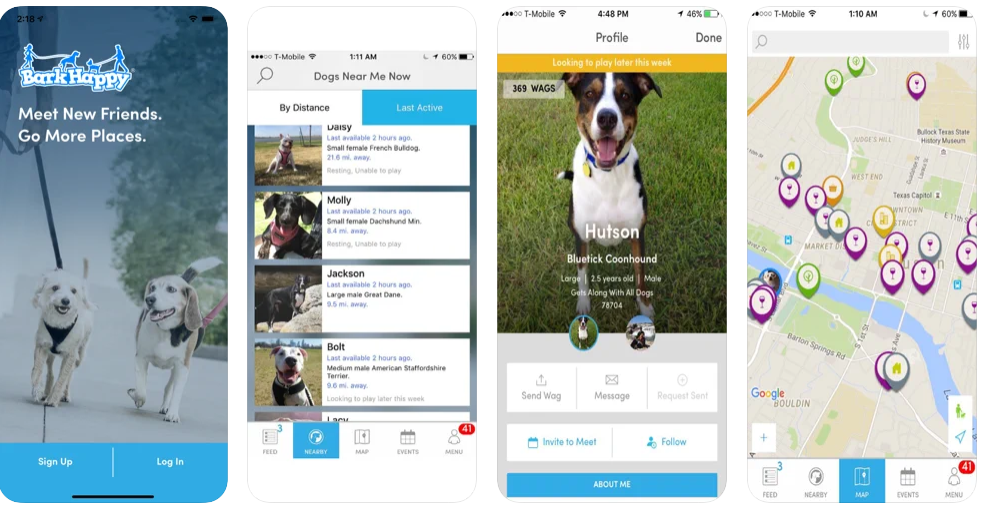
\includegraphics[scale=0.4]{slike/BarkHappy.PNG} %veličina slike u odnosu na originalnu datoteku i pozicija slike
			\centering
			\caption{BarkHappy}
			\label{fig:promjene}
		\end{figure}
	
		\par Yummypets je web i mobilna aplikacija za vlasnike kućnih ljubimaca svih vrsta, s naglaskom na dijeljenje fotografija i videa u stilu Instagrama. Aplikacija je vrlo sličnih funkcionalnosti kao projektni zadatak, a najveće razlike su postojanje dediciranog foruma i funkcije pronalaska najbliže veterinarske postaje.
		
		\begin{figure}[H]
			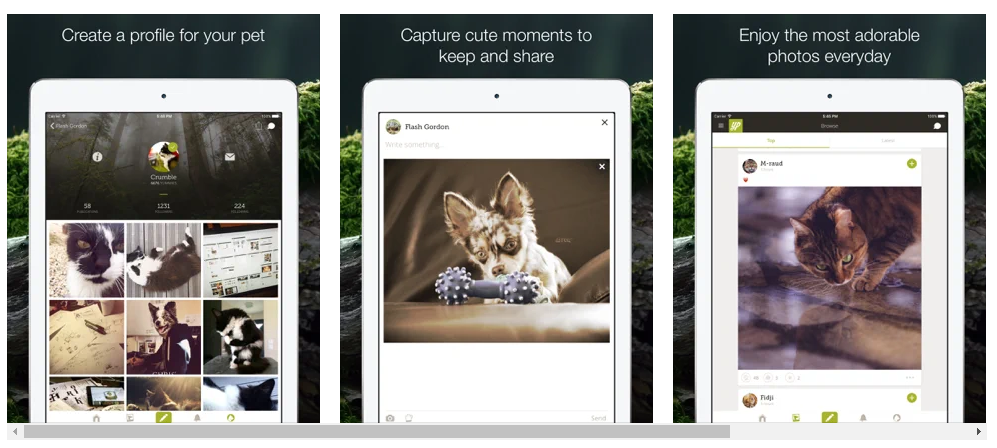
\includegraphics[scale=0.4]{slike/Yummypets.PNG} %veličina slike u odnosu na originalnu datoteku i pozicija slike
			\centering
			\caption{Yummypets}
			\label{fig:promjene}
		\end{figure}
	
		\par Cilj projektnog zadatka je aplikacija "Naši Ljubimci". Zamišljena je kao društvena mreža za vlasnike kućnih ljubimaca i tvrtke koje pružaju usluge vezane uz skrb o ljubimcima. Za korištenje aplikacije nužna je registracija korisnika. Potrebni osobni podaci su:
		
		
		\begin{packed_item}
			\item ime
			\item prezime
			\item adresa e-pošte
			\item željeno korisničko ime
		\end{packed_item}
		
		\par Tijekom registracije, korisnik mora odabrati jednu od željenih kategorija: vlasnik ljubimca ili tvrtka (obrt). 
		\par \underbar{Vlasnik ljubimca} može uređivati vlastiti profil, što podrazumjeva promjenu profilne fotografije, promjenu adrese e-pošte te stvaranje profila svojih ljubimaca. Svaki ljubimac unutar vlasnikovog profila ima svoj zaseban profil. Kategorije kućnih ljubimaca su sljedeće:
		
		\begin{packed_item}
			\item psi
			\item mačke
			\item mali glodavci
			\item ptice
			\item gmazovi
			\item egzotično 
		\end{packed_item}
	
		\par Za pojedinog ljubimca potrebno je unijeti ime, dob, spol, profilnu fotografiju i kratki opis. Za pse i mačke potrebno je dodatno evidentirati pasmina, a za sve ostale kategorije potrebno je evidentirati točnu vrstu životinje. Sve profile ljubimaca je moguće naknadno uređivati (promjena osnovnih podataka te profilne fotografije) te je moguće objavljivati fotografije i video uratke o ljubimcu uz kratak opis objave. U sklopu medijske galerije, vlasnici na svom profilu mogu objavljivati foto i video materijale s kratkim opisom (poput zajedničkih fotografija s jednim ili više ljubimaca). Vlasnici mogu poslati zahtjev za prijateljstvom drugim vlasnicima, koji ga onda mogu prihvatiti, odbiti ili trajno blokirati. Prijatelji međusobno vide medijske galerije te mogu ostavljati kratke komentare. Vlasnik profila ima pravo brisanja neželjenih komentara te prekida prijateljstva. Aplikacija podržava kreiranje događaja (evenata). Svaki vlasnik može stvoriti novi događaj, kojim će ostale vlasnike potenicijalno potaknuti na druženje. Svaki novi događaj mora sadržavati:
		
		\begin{packed_item}
			\item datum
			\item trajanje
			\item lokaciju 
			\item opis
		\end{packed_item}
		Dogovaranje sastanaka unutar Naši Ljubimci, bit će povezano s Google Calendar sustavom zbog lakše potvrde dolaska (RVSP). Vlasnik događaj može dijeliti samo s prijateljima ili sa svim registriranim korisnicima. Svi korisnici kojima je događaj vidljiv imaju opciju odabira statusa dolaska: 
		\begin{packed_item}
			\item "dolazim"
			\item "možda"
			\item "ne dolazim" 
		\end{packed_item}
		Također je moguće ostaviti kratki komentar na događaj.
		
		\par \underbar{Tvrtka (obrt)} na svom profilu prijavljuje jednu ili više od dostupnih usluga:
		\begin{packed_item}
			\item čuvanje
			\item odgoj
			\item briga o zdravlju 
		\end{packed_item}
		Podaci o tvrki (naziv, adresa, kontakt) na njenom profilu vidljivi su svim registriranim korisnicima, uz detaljan opis ponuđenih usluga. Tvrtke na svom profilu mogu objavljivati foto i video materijale te kratke poruke na koje svi korisnici mogu odgovarati. Tvrtke također mogu stvarati nove događaje, na koje se mogu prijaviti svi korisnici aplikacije.
		
		\par Svi korisnici aplikacije mogu pretraživati druge korisnike te si međusobno slati direktne poruke. U slučaju zlouporabe aplikacije, svi korisnici mogu prijaviti drugog korisnika ili tvrtku administratoru.
		
		\par \underbar {Administratori} aplikacije nemaju javne profile, niti se tretiraju kao vlasnici ljubimaca. Oni imaju mogućnost blokiranja ili trajnog brisanja profila korisnika, ukoliko se za to pojavi potreba.
		
		\par Ovaj sustav ima velikog potencijala za proširenje i nadogradnju. Evo nekoliko ideja za budućnost:
		\begin{packed_item}
			\item \textit {end-to-end} enkripcija direktnih poruka za veću privatnost
			\item 2-faktorska autentikacija za bolju sigurnost
			\item predlaganje novih prijatelja na temelju geolokacije
			\item dodavanje \textit {feeda} s novim objavama korisnikovih prijatelja
			\item dodavanje mogućnosti plaćenih oglasa u vidu istaknutih objava za tvrtke i obrte
		\end{packed_item}
		
		
		\eject
		
		
	
	\chapter{Specifikacija programske potpore}
		
	\section{Funkcionalni zahtjevi}
			
			\noindent \textbf{Dionici:}
			
			\begin{packed_enum}
				
				\item Vlasnik životinje
				\item Tvrtka				
				\item Administrator
				\item Razvojni tim
				
			\end{packed_enum}
			
			\noindent \textbf{Aktori i njihovi funkcionalni zahtjevi:}
			
			
			\begin{packed_enum}
				\item  \underbar{Neregistrirani/neprijavljeni korisnik može:}
				
				\begin{packed_enum}
					
					\item Pregledavati početnu stranicu platforme Naši ljubimci.
					\item Registrirati se na platformu Naši ljubimci.
					
				\end{packed_enum}
			
				\item  \underbar{Prijavljeni korisnik, vlasnik životinje može:}
				
				\begin{packed_enum}
					
					\item Uređivati vlastiti korisnički profil.
					\item Kreirati profil za svojeg ljubimca.
					\item Uređivati profil ljubimca.
					\item Objavljivati foto I video materijale uz kratki opis na profilu svojega ljubimca.
					\item Objavljivati foto I video materijale uz kratki opis u medijskim galerijama vlastitih profila.
					\item Komentirati na medijskim galerijama profila drugih vlasnika ljubimaca.
					\item Komentirati objevljene sadržaje na profilu tvrtki.
					\item Slati zahtjeve za prijateljstvo.
					\item Prihvatiti ili odbiti zahtjev za prijateljstvo ili pak trajno blokirati pošiljatelja zahtjeva. 
					\item Kreirati događaje.
					\item Navesti status uz sebi vidljive događaje.
					\item Pretraživati korisnike.
					\item Slati izravne poruke.
					\item Prijaviti korisnika administratoru.
					
				\end{packed_enum}
			
				\item  \underbar{Prijavljeni korisnik, tvrtka može:}
				
				\begin{packed_enum}
					
					\item Objavljivati kratke poruke, foto I video materijale na vlastitom profilu.
					\item Kreirati nove događaje.
					\item Slati izravne poruke.
					
				\end{packed_enum}
			
				\item  \underbar{Administrator može:}
				
				\begin{packed_enum}
					
					\item Privremeno blokirati registriranog korisnika, vlasnika ili tvrtku.
					\item Trajno izbrisati korisnički račun. 
					
				\end{packed_enum}
				
			\end{packed_enum}
			
			\eject 
			
			
				
			\subsection{Obrasci uporabe}
				
				
				\subsubsection{Opis obrazaca uporabe}

					\noindent \underbar{\textbf{UC1 - Pregled stranice}}
					\begin{packed_item}
	
						\item \textbf{Glavni sudionik: } Korisnik
						\item  \textbf{Cilj:} Pregled stranice Naši ljubimci
						\item  \textbf{Sudionici:} Baza podataka
						\item  \textbf{Preduvjet:} -
						\item  \textbf{Opis osnovnog tijeka:}
						
						\item[] \begin{packed_enum}
	
							\item Neregistrirani ili neprijavljeni korisnik u web pregledniku pregledava stranicu platforme Naši ljubimci 
			
						\end{packed_enum}
						
					\end{packed_item}
				
				\noindent \underbar{\textbf{UC2 - Registracija, vlasnik}}
				\begin{packed_item}
					
					\item \textbf{Glavni sudionik: } Korisnik
					\item  \textbf{Cilj:} Registracija na platformi Naši ljubimci
					\item  \textbf{Sudionici:} Baza podataka
					\item  \textbf{Preduvjet:} -
					\item  \textbf{Opis osnovnog tijeka:}
					
					\item[] \begin{packed_enum}
						
						\item Unos registracijskih podataka (ime, prezime, e-mail adresa, korisničko ime)
						\item Potvrda o ispravnosti unesenih podataka
						\item Spremanje podataka u bazu podataka
						\item Pristup korisničkim funkcijama
					\end{packed_enum}
					
					\item  \textbf{Opis mogućih odstupanja:}
					
					\item[] \begin{packed_item}
						
						\item[2.a] Zauzeto korisničko ime/e-mail
						\item[] \begin{packed_enum}
							\item Sustav obavještava korisnika o neuspjeloj registraciji i vraća  ga na stranicu za unos registracijskih podataka
							
						\end{packed_enum}
						
					\end{packed_item}
				\end{packed_item}
				
				\noindent \underbar{\textbf{UC3 - Registracija, tvrtka}}
				\begin{packed_item}
					
					\item \textbf{Glavni sudionik: } Korisnik
					\item  \textbf{Cilj:} Registracija na platformi Naši ljubimci
					\item  \textbf{Sudionici:} Baza podataka
					\item  \textbf{Preduvjet:} -
					\item  \textbf{Opis osnovnog tijeka:}
					
					\item[] \begin{packed_enum}
						
						\item Unos registracijskih podataka (ime, prezime, e-mail adresa, korisničko ime)
						\item Potvrda o ispravnosti unesenih podataka
						\item Spremanje podataka u bazu podataka
						\item Pristup korisničkim funkcijama
					\end{packed_enum}
					
					\item  \textbf{Opis mogućih odstupanja:}
					
					\item[] \begin{packed_item}
						
						\item[2.a] Zauzeto korisničko ime/e-mail
						\item[] \begin{packed_enum}
							
							\item Sustav obavještava korisnika o neuspjeloj registraciji i vraća  ga na stranicu za unos registracijskih podataka
							
						\end{packed_enum}
						
					\end{packed_item}
				\end{packed_item}
				
				\noindent \underbar{\textbf{UC4 - Prijava}}
				\begin{packed_item}
					
					\item \textbf{Glavni sudionik: } Vlasnik, tvrtka
					\item  \textbf{Cilj:} Prijava na platformi Naši ljubimci
					\item  \textbf{Sudionici:} Baza podataka
					\item  \textbf{Preduvjet:} Registracija na platformi Naši ljubimci 
					\item  \textbf{Opis osnovnog tijeka:}
					
					\item[] \begin{packed_enum}
						
						\item Unos korisničkog imena i lozinke
						\item Potvrda o ispravnosti korisničkih podataka
						\item Pristup korisničkim funkcijama
						
					\end{packed_enum}
					
					\item  \textbf{Opis mogućih odstupanja:}
					
					\item[] \begin{packed_item}
						
						\item[2.a] Neispravno korisničko ime/lozinka
						\item[] \begin{packed_enum}
							
							\item Sustav obavještava korisnika o neuspjeloj prijavi i vraća ga na 		stranicu za unos korisničkog imena i lozinke	
							
						\end{packed_enum}	
					\end{packed_item}
				\end{packed_item}
				
				\noindent \underbar{\textbf{UC5 - Uređivanje profila, vlasnik}}
				\begin{packed_item}
					
					\item \textbf{Glavni sudionik: } Vlasnik 
					\item  \textbf{Cilj:} Izmjena korisničkog profila
					\item  \textbf{Sudionici:} Baza podataka
					\item  \textbf{Preduvjet:} Prijava u sustav
					\item  \textbf{Opis osnovnog tijeka:}
					
					\item[] \begin{packed_enum}
						
						\item Korisnik odabire opciju za uređivanje profila
						\item Otvara se stranica za mijenjanje osobnih podataka
						\item Korisnik mijenja željene podatke
						\item Korisnik sprema promjene
						\item Baza podataka se ažurira
					\end{packed_enum}
					
					\item  \textbf{Opis mogućih odstupanja:}
					
					\item[] \begin{packed_item}
						
						\item[3.a] Korisnik promijeni svoje osobne podatke, ali ne odabere opciju za spremanje promjena
						\item[] \begin{packed_enum}
							
							\item Sustav obavještava korisnika da nije spremio podatke prije izlaska iz prozora
							
						\end{packed_enum}
					\end{packed_item}
				\end{packed_item}
				
				\noindent \underbar{\textbf{UC6 - Uređivanje profila, tvrka}}
				\begin{packed_item}
					
					\item \textbf{Glavni sudionik: } Tvrtka
						\item  \textbf{Cilj:} Izmjena korisničkog profila
					\item  \textbf{Sudionici:} Baza podataka
					\item  \textbf{Preduvjet:} Prijava u sustav
					\item  \textbf{Opis osnovnog tijeka:}
					
					\item[] \begin{packed_enum}
						
						\item Korisnik odabire opciju za uređivanje profila
						\item Otvara se stranica za mijenjanje osobnih podataka
						\item Korisnik mijenja željene podatke
						\item Korisnik sprema promjene
						\item Baza podataka se ažurira
					\end{packed_enum}
					
					\item  \textbf{Opis mogućih odstupanja:}
					
					\item[] \begin{packed_item}
						
						\item[3.a] Korisnik promijeni svoje osobne podatke, ali ne odabere opciju za spremanje promjena
						\item[] \begin{packed_enum}
							
							\item Sustav obavještava korisnika da nije spremio podatke prije izlaska iz prozora
							
						\end{packed_enum}
					\end{packed_item}
				\end{packed_item}
				
				\noindent \underbar{\textbf{UC7 - Stvaranje profila ljubimca}}
				\begin{packed_item}
					
					\item \textbf{Glavni sudionik: } Vlasnik
					\item  \textbf{Cilj:} Stvaranje profila ljubimca
					\item  \textbf{Sudionici:} Baza podataka
					\item  \textbf{Preduvjet:} Prijava u sustav
					\item  \textbf{Opis osnovnog tijeka:}
					
					\item[] \begin{packed_enum}
						
						\item Korisnik u aplikaciji odabire ”Dodaj ljubimca”
						\item Otvara se obrazac za popunjavanje informacija o ljubimcu
						\item Korisnik predaje obrazac
						\item Baza podataka se ažurira
						
					\end{packed_enum}
					
					\item  \textbf{Opis mogućih odstupanja:}
					
					\item[] \begin{packed_item}
						
						\item[3.a] Korisnik predaje obrazac koji nije u potpunosti ispunjen
						\item[] \begin{packed_enum}
							
							\item Sustav obavještava korisnika da mora ispuniti obrazac prije predaje
							
						\end{packed_enum}					
					\end{packed_item}
				\end{packed_item}
				
				\noindent \underbar{\textbf{UC8 - Uređivanje profila ljubimca}}
				\begin{packed_item}
					
					\item \textbf{Glavni sudionik: } Vlasnik
					\item  \textbf{Cilj:} Izmjena profilnih podataka
					\item  \textbf{Sudionici:} Baza podataka
					\item  \textbf{Preduvjet:} Prijava u sustav
					\item  \textbf{Opis osnovnog tijeka:}
					
					\item[] \begin{packed_enum}
						
						\item Korisnik odabire opciju za uređivanje profila na stranici ljubimca
						\item Otvara se stranica za mijenjanje podataka ljubimca
						\item Korisnik mijenja željene podatke
						\item Korisnik sprema promjene
						\item Baza podataka se ažurira
					\end{packed_enum}
					
					\item  \textbf{Opis mogućih odstupanja:}
					
					\item[] \begin{packed_item}
						
						\item[3.a] Korisnik promijeni svoje osobne podatke, ali ne odabere opciju za spremanje promjena
						\item[] \begin{packed_enum}
							
							\item Sustav obavještava korisnika da nije spremio podatke prije izlaska iz prozora							
							
						\end{packed_enum}						
					\end{packed_item}
				\end{packed_item}
				
				\noindent \underbar{\textbf{UC9 - Uređivanje profila ljubimca}}
				\begin{packed_item}
					
					\item \textbf{Glavni sudionik: } Vlasnik
					\item  \textbf{Cilj:} Objava foto ili video materijala 
					\item  \textbf{Sudionici:} Baza podataka
					\item  \textbf{Preduvjet:} Prijava u sustav
					\item  \textbf{Opis osnovnog tijeka:}
					
					\item[] \begin{packed_enum}
						
						\item Korisnik odabire opciju dodavanja medijskog sadržaja 
						\item Otvara se stranica za dodavanje videa ili fotografija
						\item Korisnik dodaje video ili fotografiju
						\item Korisnik sprema promjene
						\item Baza podataka se ažurira
					\end{packed_enum}
					
					\item  \textbf{Opis mogućih odstupanja:}
					
					\item[] \begin{packed_item}
						
						\item[3.a] Korisnik dodaje sadržaj, ali ne odabere opciju za spremanje promjena
						\item[] \begin{packed_enum}
							
							\item Sustav obavještava korisnika da nije spremio podatke prije izlaska iz prozora
							
						\end{packed_enum}						
					\end{packed_item}
				\end{packed_item}
				
				\noindent \underbar{\textbf{UC10 - Osobni profil, objava foto i video materijala}}
				\begin{packed_item}
					
					\item \textbf{Glavni sudionik: } Vlasnik, tvrtka
					\item  \textbf{Cilj:} Objava kratkih poruka, foto ili video materijala 
					\item  \textbf{Sudionici:} Baza podataka
					\item  \textbf{Preduvjet:} Prijava u sustav
					\item  \textbf{Opis osnovnog tijeka:}
					
					\item[] \begin{packed_enum}
						
						\item Korisnik odabire opciju dodavanja medijskog sadržaja 
						\item Otvara se stranica za dodavanje videa ili fotografija
						\item Korisnik dodaje video ili fotografiju
						\item Korisnik sprema promjene
						\item Baza podataka se ažurira
					\end{packed_enum}
					
					\item  \textbf{Opis mogućih odstupanja:}
					
					\item[] \begin{packed_item}
						
						\item[3.a] Korisnik dodaje sadržaj, ali ne odabere opciju za spremanje promjena
						\item[] \begin{packed_enum}
							
							\item Sustav obavještava korisnika da nije spremio podatke prije izlaska iz prozora
							
						\end{packed_enum}
					\end{packed_item}
				\end{packed_item}
			
				
				\noindent \underbar{\textbf{UC11 - Komentiranje na profilu tvrtke}}
				\begin{packed_item}
					
					\item \textbf{Glavni sudionik: } Vlasnik
					\item  \textbf{Cilj:} Komentiranje objavljenih sadržaja na profilu tvrtke
					\item  \textbf{Sudionici:} Baza podataka
					\item  \textbf{Preduvjet:} Prijava u sustav
					\item  \textbf{Opis osnovnog tijeka:}
					
					\item[] \begin{packed_enum}
						
						\item Korisnik odabire opciju dodavanja komentara na sadržaj
						\item Otvara se prozor za upisivanje komentara
						\item Korisnik upisuje komentar
						\item Korisnik sprema promjene
						\item Baza podataka se ažurira
					\end{packed_enum}
					
					\item  \textbf{Opis mogućih odstupanja:}
					
					\item[] \begin{packed_item}
						
						\item[3.a] Korisnik upisuje komentar, ali ne odabere opciju za objavu
						\item[] \begin{packed_enum}
							
							\item Sustav obavještava korisnika da komentar pri promjeni stranice neće biti spremljen
							
						\end{packed_enum}
						
					\end{packed_item}
				\end{packed_item}
				
				\noindent \underbar{\textbf{UC12 - Slanje zahtjeva za prijateljstvo}}
				\begin{packed_item}
					
					\item \textbf{Glavni sudionik: } Vlasnik
					\item  \textbf{Cilj:} Slanje zahtjeva za prijateljsvo drugim vlasnicima
					\item  \textbf{Sudionici:} Baza podataka
					\item  \textbf{Preduvjet:} Prijava u sustav
					\item  \textbf{Opis osnovnog tijeka:}
					
					\item[] \begin{packed_enum}
						
						\item Korisnik otvara profil drugog korisnika 
						\item Korisnik pritisne gumb ”Dodaj prijatelja”
						\item Baza podataka se ažurira
					\end{packed_enum}
					
					\item  \textbf{Opis mogućih odstupanja:}
					
					\item[] \begin{packed_item}
						
						\item[2.a] Drugi korisnik odgovara na zahtjev za prijateljstvo
						\item[] \begin{packed_enum}
							
							\item Korisnik odgovara s "Prihvati zahtjev"
							\item Korisnik odgovara s "Odbij zahtjev"
							\item Korisnik odgovara s "Blokiraj"
							
						\end{packed_enum}
					\end{packed_item}
				\end{packed_item}
				
				\noindent \underbar{\textbf{UC13 - Komentiranje u medijskoj galeriji}}
				\begin{packed_item}
					
					\item \textbf{Glavni sudionik: } Vlasnik
					\item  \textbf{Cilj:} Objava kratkog komentara u medijskoj galeriji
					\item  \textbf{Sudionici:} Baza podataka
					\item  \textbf{Preduvjet:} Prijava u sustav, prijateljsvo s vlasnikom pripadne medijske galerije
					\item  \textbf{Opis osnovnog tijeka:}
					
					\item[] \begin{packed_enum}
						
						\item Korisnik odabire opciju dodavanja komentara na sadržaj
						\item Otvara se prozor za upisivanje komentara
						\item Korisnik upisuje komentar
						\item Korisnik sprema promjene
						\item Baza podataka se ažurira
					\end{packed_enum}
					
					\item  \textbf{Opis mogućih odstupanja:}
					
					\item[] \begin{packed_item}
						
						\item[3.a] Korisnik upisuje komentar, ali ne odabere opciju za objavu
						\item[] \begin{packed_enum}
							
							\item Sustav obavještava korisnika da komentar pri promjeni stranice neće biti objavljen
							
						\end{packed_enum}
						
					\end{packed_item}
				\end{packed_item}
				
				\noindent \underbar{\textbf{UC14 - Brisanje komentara}}
				\begin{packed_item}
					
					\item \textbf{Glavni sudionik: } Vlasnik
					\item  \textbf{Cilj:} Brisanje neželjenih komentara
					\item  \textbf{Sudionici:} Baza podataka
					\item  \textbf{Preduvjet:} Prijava u sustav
					\item  \textbf{Opis osnovnog tijeka:}
					
					\item[] \begin{packed_enum}
						
						\item Korisnik odabire željeni komentar
						\item Korisnik odabire brisanje komentara
						\item Baza podataka se ažurira
					\end{packed_enum}
					
				\end{packed_item}
				
				\noindent \underbar{\textbf{UC15 - Raskid prijateljstva}}
				\begin{packed_item}
					
					\item \textbf{Glavni sudionik: } Vlasnik
					\item  \textbf{Cilj:} Raskid prijateljstva  s drugim vlasnikom
					\item  \textbf{Sudionici:} Baza podataka
					\item  \textbf{Preduvjet:} Prijava u sustav, uspostavljeno prijateljstvo s drugim vlasnikom
					\item  \textbf{Opis osnovnog tijeka:}
					
					\item[] \begin{packed_enum}
						
						\item Korisnik odabire drugoga korisnika 
						\item Korisnik odabire raskid prijateljstva 
						\item Baza podataka se ažurira
					\end{packed_enum}
					
				\end{packed_item}
				
				\noindent \underbar{\textbf{UC16 - Kreiranje događaja}}
				\begin{packed_item}
					
					\item \textbf{Glavni sudionik: } Vlasnik, tvrtka
					\item  \textbf{Cilj:} Kreiranje događaja
					\item  \textbf{Sudionici:} Baza podataka
					\item  \textbf{Preduvjet:} Prijava u sustav
					\item  \textbf{Opis osnovnog tijeka:}
					
					\item[] \begin{packed_enum}
						
						\item Korisnik odabire opciju kreiranja događaja
						\item Otvara se obrazac za popunjavanje informacija o događaju
						\item Korisnik predaje obrazac
						\item Baza podataka se ažurira
					\end{packed_enum}
					
					\item  \textbf{Opis mogućih odstupanja:}
					
					\item[] \begin{packed_item}
						
						\item[3.a] Već postoji događaj s istim sadržajem
						\item[] \begin{packed_enum}
							
							\item Sustav obavještava korisnika o već postojećem događaju i vraća ga na popunjavanje obrasca
							
						\end{packed_enum}
					\end{packed_item}
				\end{packed_item}
			
				\noindent \underbar{\textbf{UC17 - Pretraživanje}}
				\begin{packed_item}
					
					\item \textbf{Glavni sudionik: } Vlasnik  
					\item  \textbf{Cilj:} Pretraga drugih korisnika
					\item  \textbf{Sudionici:} Baza podataka
					\item  \textbf{Preduvjet:} Prijava u sustav
					\item  \textbf{Opis osnovnog tijeka:}
					
					\item[] \begin{packed_enum}
						
						\item Korisnik odabire opciju pretraživanja
						\item Korisnik upisuje ime korisnika ili tvrtke koju želi pronaći
						\item Prikazuju se rezultati pretrage
					\end{packed_enum}
					
					\item  \textbf{Opis mogućih odstupanja:}
					
					\item[] \begin{packed_item}
						
						\item[2.a] Ne postoji korisnik ili tvrtka pod tim imenom
						\item[] \begin{packed_enum}
							
							\item Sustav obavještava korisnika da nema rezultata takve pretrage
							
						\end{packed_enum}
						
					\end{packed_item}
				\end{packed_item}	
				
				\noindent \underbar{\textbf{UC18 - Prijava na događaj}}
				\begin{packed_item}
					
					\item \textbf{Glavni sudionik: } Vlasnik
					\item  \textbf{Cilj:} Navođenje statusa uz događaj
					\item  \textbf{Sudionici:} Baza podataka
					\item  \textbf{Preduvjet:} Prijava u sustav, vidljivost događaja
					\item  \textbf{Opis osnovnog tijeka:}
					
					\item[] \begin{packed_enum}
						
						\item Korisnik odabire željeni događaj
						\item Korisnik odabire jednu od opcija dolaska na događaj
						\item Baza podataka se ažurira

					\end{packed_enum}
					
					\item  \textbf{Opis mogućih odstupanja:}
					
				\end{packed_item}
				
				
				\noindent \underbar{\textbf{UC19 - Slanje poruke}}
				\begin{packed_item}
					
					\item \textbf{Glavni sudionik: } Vlasnik
					\item  \textbf{Cilj:} Slanje direktne poruke	
					\item  \textbf{Sudionici:} Baza podataka
					\item  \textbf{Preduvjet:} Prijava u sustav
					\item  \textbf{Opis osnovnog tijeka:}
					
					\item[] \begin{packed_enum}
						
						\item Korisnik se pozicionira na profil drugog korisnika 
						\item Korisnik odabire opciju ”Poruka”
						\item Korisnik upisuje željenu poruku
						\item Korisnik odabire ”Slanje poruke”
						\item Baza podataka se ažurira
					\end{packed_enum}
					
				\end{packed_item}
				
				\noindent \underbar{\textbf{UC20 - Prijava}}
				\begin{packed_item}
					
					\item \textbf{Glavni sudionik: } Vlasnik
					\item  \textbf{Cilj:} Prijava drugog korisnika ili tvrtke
					\item  \textbf{Sudionici:} Baza podataka
					\item  \textbf{Preduvjet:} Prijava u sustav
					\item  \textbf{Opis osnovnog tijeka:}
					
					\item[] \begin{packed_enum}
						
						\item Korisnik se pozicionira na profil drugog korisnika
						\item Korisnik odabire opciju ”Prijavi”
						\item Baza podataka se ažurira
					\end{packed_enum}
					
				\end{packed_item}
				
				\noindent \underbar{\textbf{UC21 - Privremeno blokiranje}}
				\begin{packed_item}
					
					\item \textbf{Glavni sudionik: } Administrator
					\item  \textbf{Cilj:} Prijava drugog korisnika ili tvrtke
					\item  \textbf{Sudionici:} Baza podataka
					\item  \textbf{Preduvjet:} Prijava u sustav
					\item  \textbf{Opis osnovnog tijeka:}
					
					\item[] \begin{packed_enum}
						
						\item Administrator pronalazi željenog korisnika
						\item Administrator odabire opciju ”Privremeno blokiraj”
						\item Baza podataka se ažurira
					\end{packed_enum}
					
				\end{packed_item}
				
				\noindent \underbar{\textbf{UC22 - Trajno brisanje}}
				\begin{packed_item}
					
					\item \textbf{Glavni sudionik: } Administrator
					\item  \textbf{Cilj:} Brisanje računa vlasnika ili tvrtke
					\item  \textbf{Sudionici:} Baza podataka
					\item  \textbf{Preduvjet:} Prijava u sustav
					\item  \textbf{Opis osnovnog tijeka:}
					
					\item[] \begin{packed_enum}
						
						\item Administrator pronalazi željenog korisnika
						\item Administrator odabire opciju ”Obriši korisnika”
						\item Baza podataka se ažurira
					\end{packed_enum}
				\end{packed_item}
						
				\subsubsection{Dijagrami obrazaca uporabe}
					\begin{figure} 
						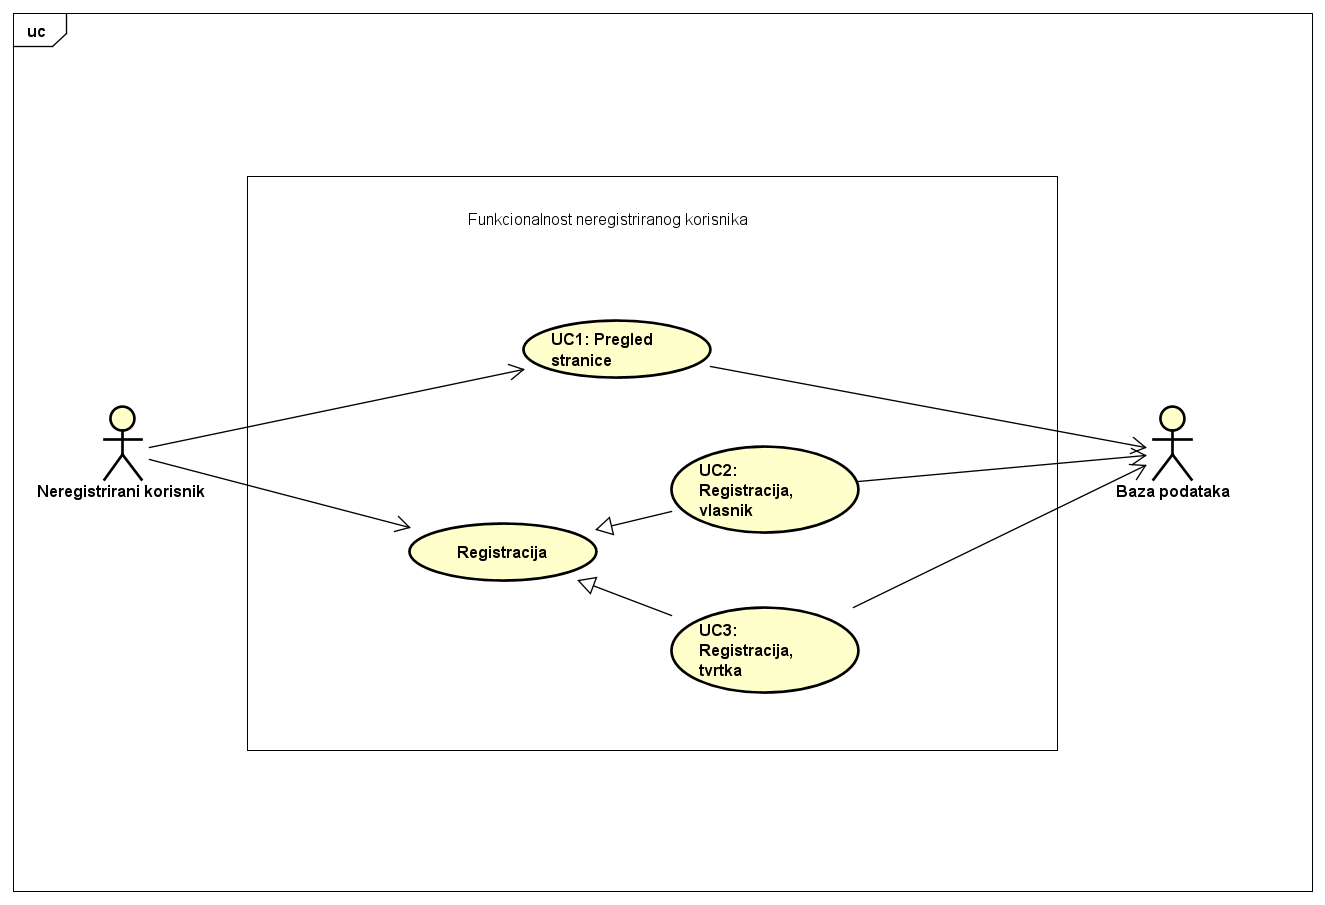
\includegraphics[width=\textwidth]{slike/funkc_neregistriranog_korisnika.png}
						\caption{Funkcionalnost neregistriranog korisnika u aplikaciji}
					\end{figure}
					\begin{figure} 
						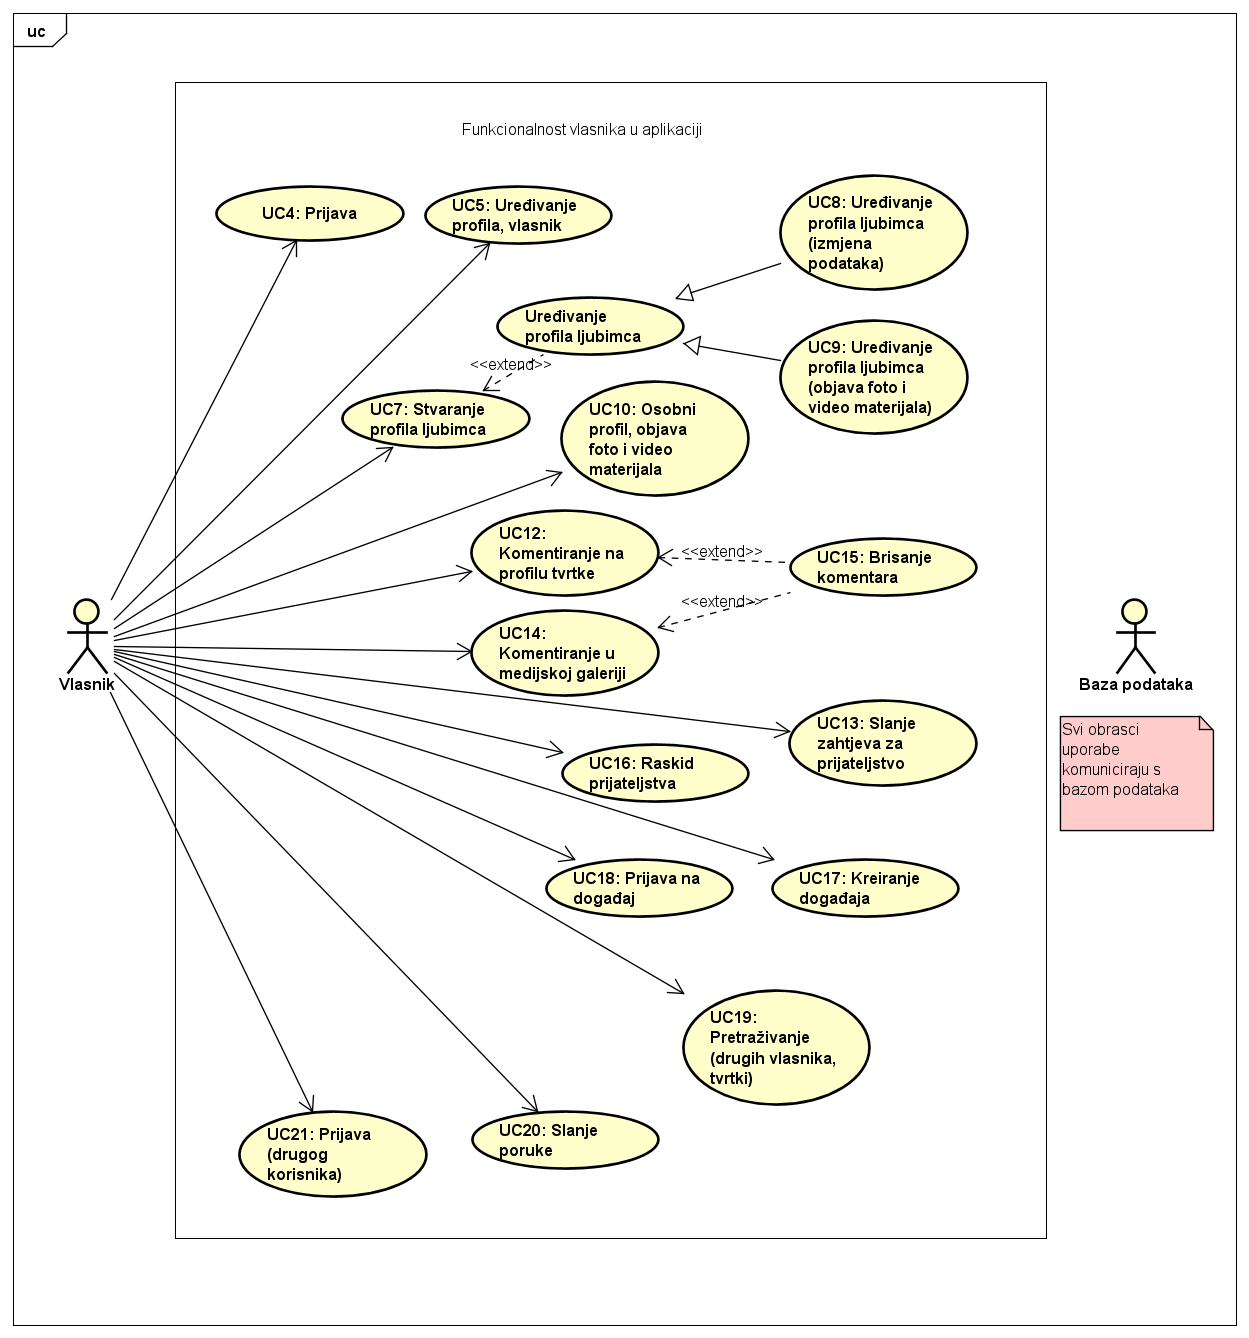
\includegraphics[width=\textwidth]{slike/funkcionalnost_vlasnika.png}
						\caption{Funkcionalnost vlasnika u aplikaciji}
					\end{figure}
					\begin{figure} 
						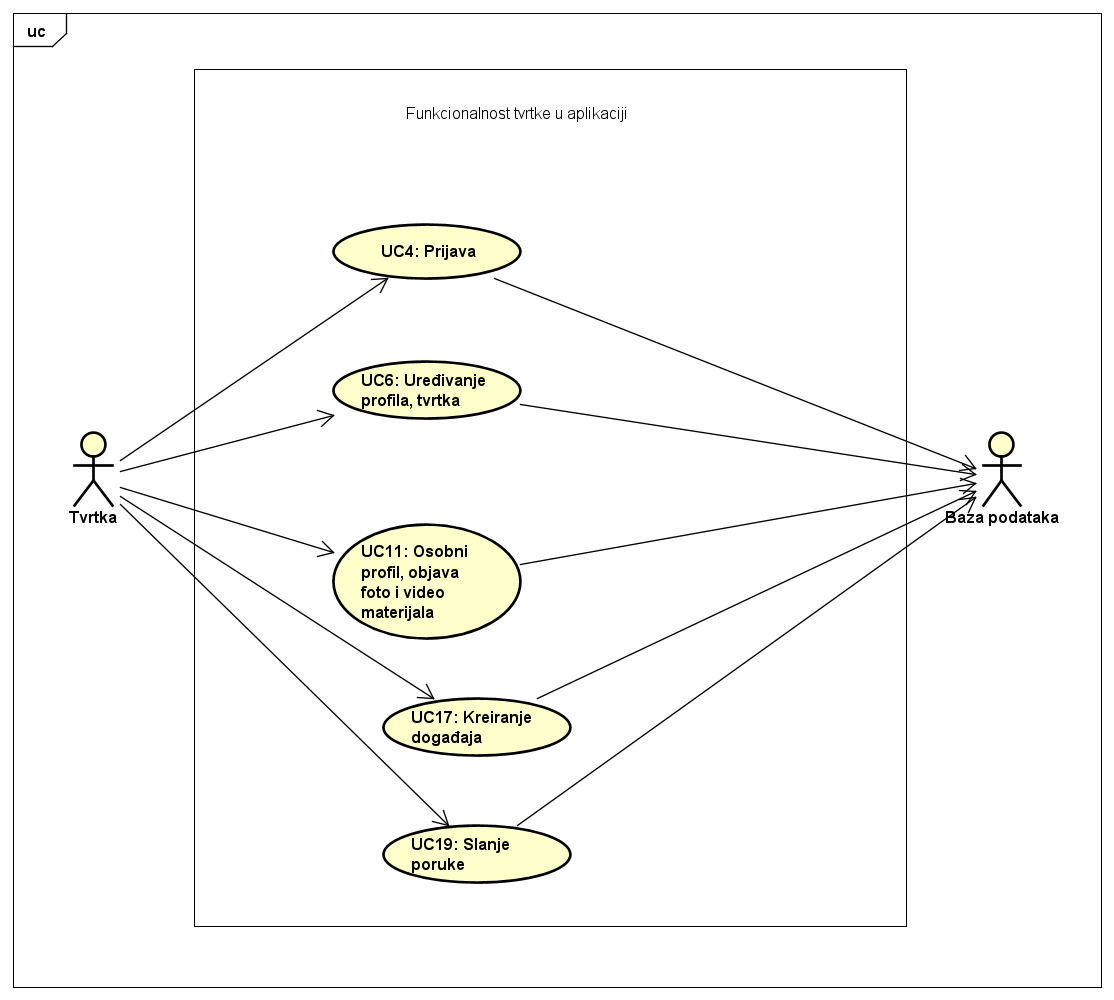
\includegraphics[width=\textwidth]{slike/funkcionalnost_tvrtke.png}
						\caption{Funkcionalnost tvrtke u aplikaciji}
					\end{figure}
					\begin{figure} 
						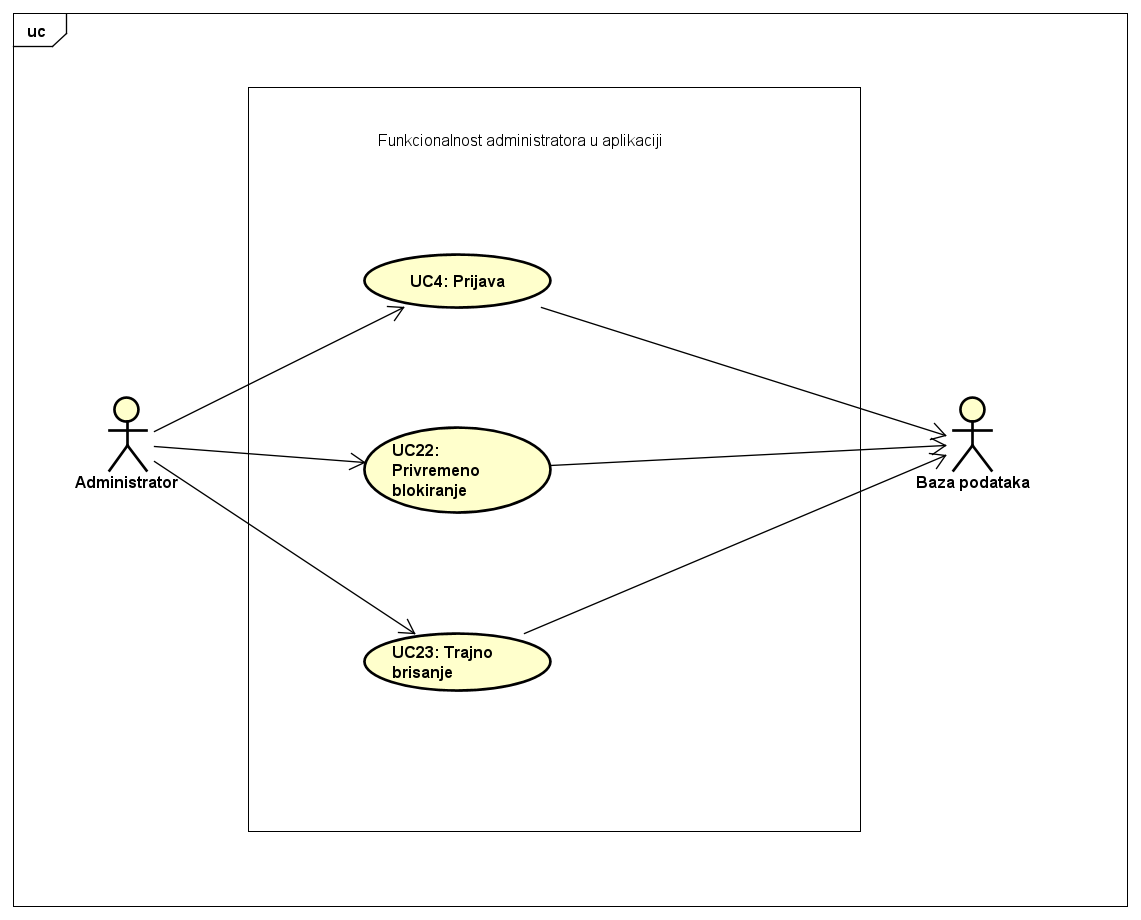
\includegraphics[width=\textwidth]{slike/funkcionalnost_administratora.png}
						\caption{Funkcionalnost administratora u aplikaciji}
					\end{figure}
				\eject		
				
			\subsection{Sekvencijski dijagrami}
				
				\textbf{Obrazac uporabe UC7 - Stvaranje profila ljubimca}\\
				\indent Vlasnik u aplikaciji odabire opciju stvaranja profila ljubimca. Otvara mu se prazan obrazac za kreiranje profila koji vlasnik ispunjava i prosljeđuje aplikaciji koja sprema podatke u bazu podataka i tako je stvoren novi profil ljubimca.
				
				\begin{figure}[H]
					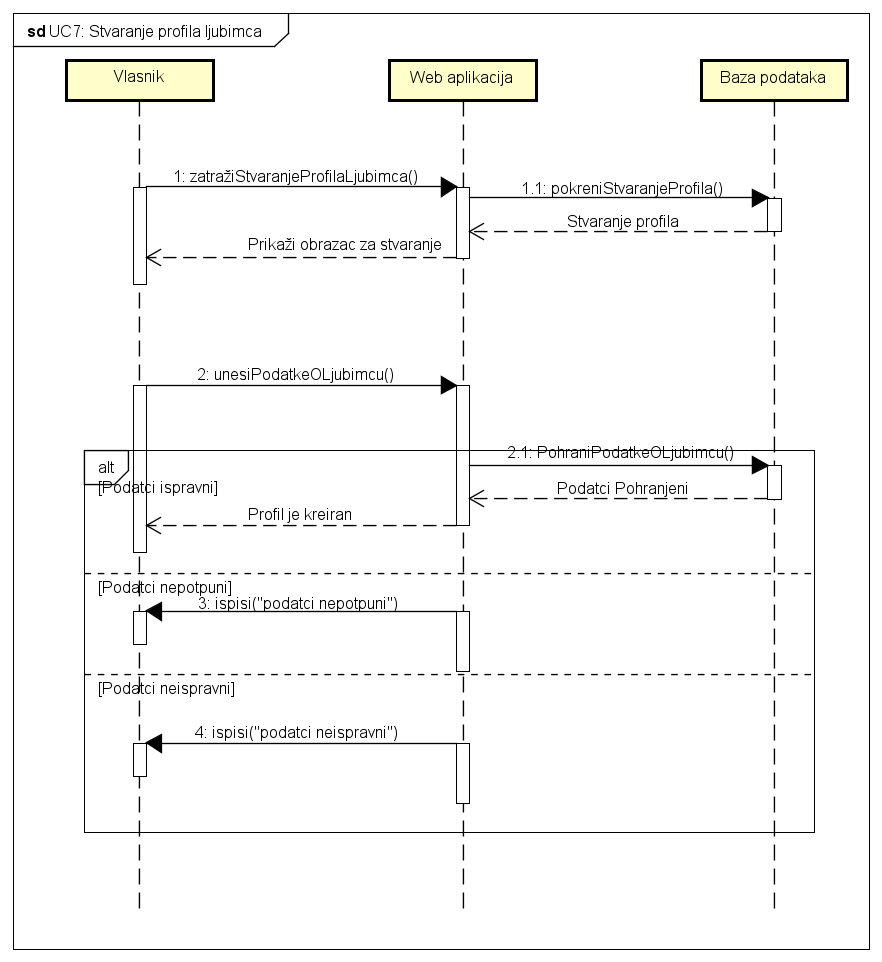
\includegraphics[scale=0.5]{slike/UC7.PNG} %veličina slike u odnosu na originalnu datoteku i pozicija slike
					\centering
					\caption{Sekvencijski dijagram za UC7}
				\end{figure}
				
				\pagebreak
				\textbf{Obrazac uporabe UC16 - Kreiranje događaja}\\
				\indent Tvrtka u aplikaciji odabire opciju kreiranja novog događaja. Otvara se obrazac za kreiranje novog događaja koji se ispunjava i prosljeđuje aplikaciji koja pohranjuje podatke u bazu podataka i kreira se novi događaj
				
				\begin{figure}[H]
					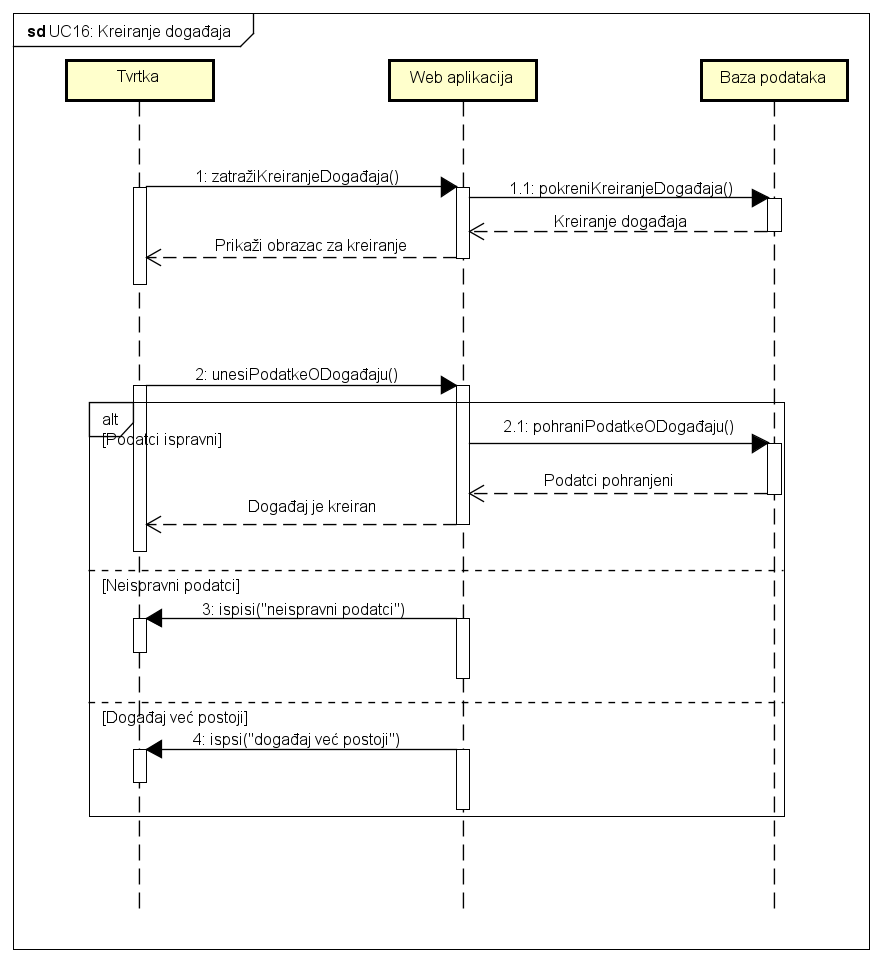
\includegraphics[scale=0.5]{slike/Uc16.PNG} %veličina slike u odnosu na originalnu datoteku i pozicija slike
					\centering
					\caption{Sekvencijski dijagram za UC17}
				\end{figure}
				
				\pagebreak
				\textbf{Obrazac uporabe UC18 - Prijava na događaj}\\
				\indent Vlasnik u aplikaciji odabire opciju prijave na događaj. Nakon odabira željenog događaja vlasnik potvrđuje prijavu i podatci se spremaju u bazu podataka. Vlasnik je prijavljen na odabrani događaj.
				
				\begin{figure}[H]
					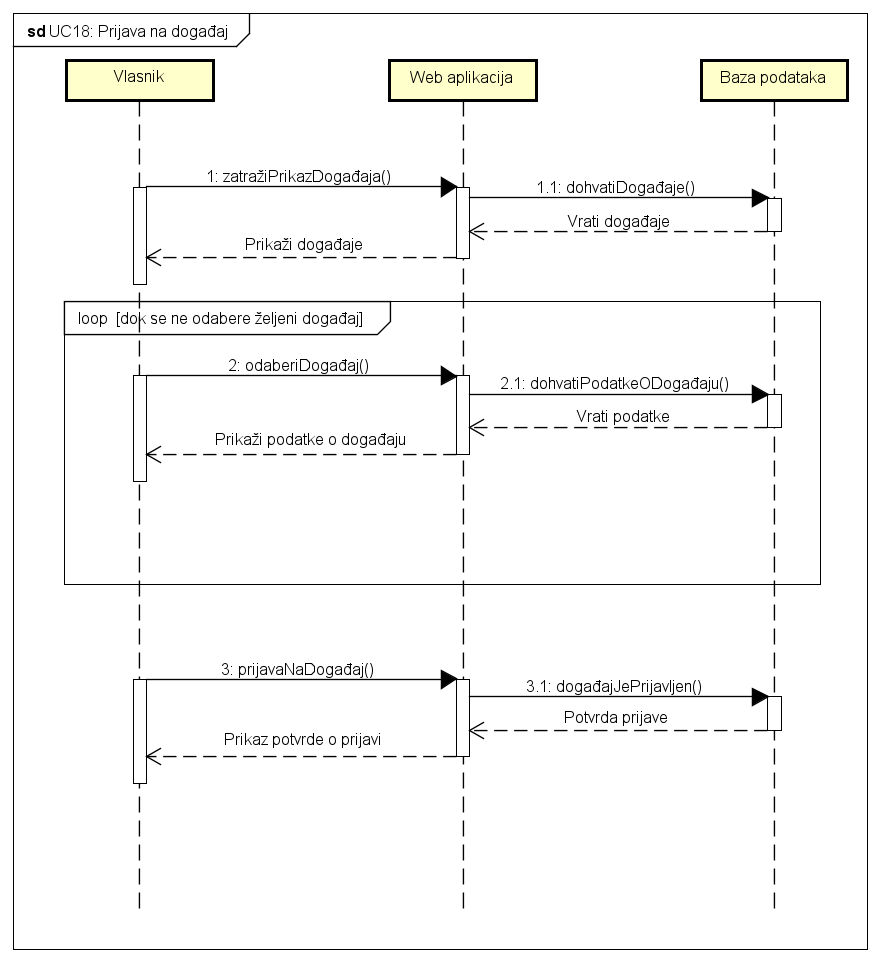
\includegraphics[scale=0.5]{slike/UC18.PNG} %veličina slike u odnosu na originalnu datoteku i pozicija slike
					\centering
					\caption{Sekvencijski dijagram za UC18}
				\end{figure}
				
				\pagebreak
				\textbf{Obrazac uporabe UC22 - Trajno brisanje}\\
				\indent Administrator u aplikaciji odabire željenog korisnika kojeg želi trajno obrisati. Potvrdom na brisanje korisnika svi njegovi podatci o računu se brišu iz baze podataka i korisnik se više ne može prijaviti u aplikaciju.
				
				\begin{figure}[H]
					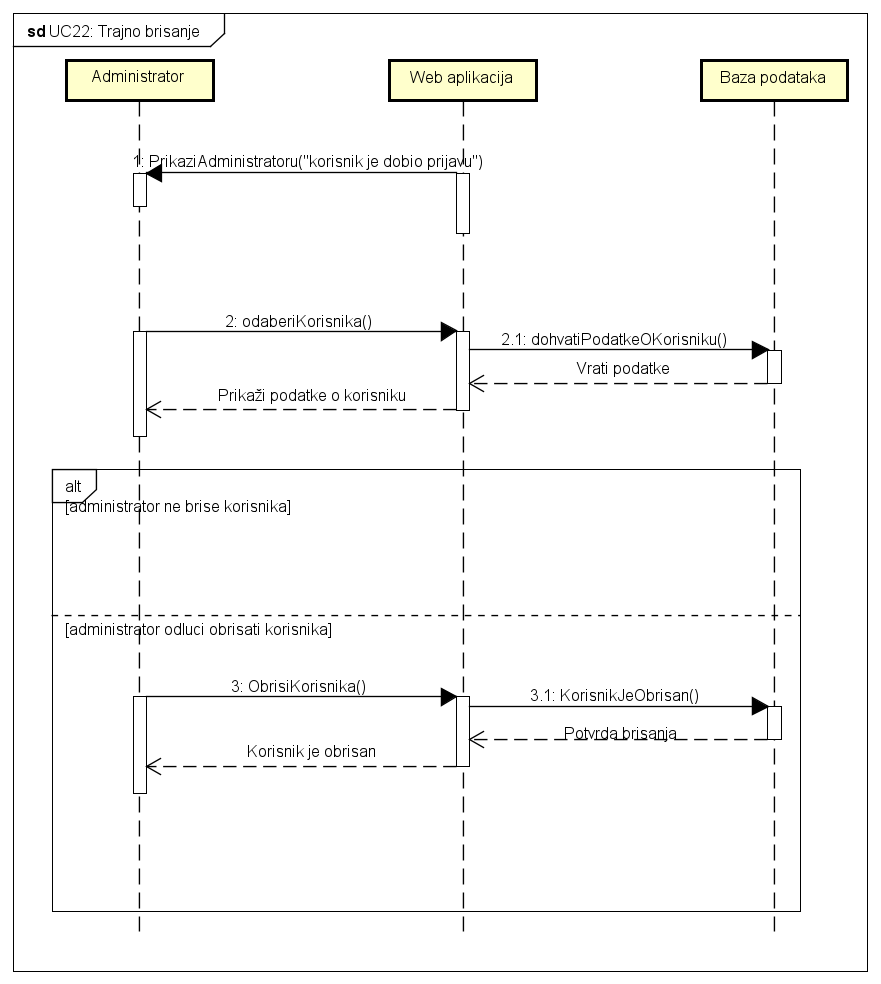
\includegraphics[scale=0.5]{slike/Uc22.PNG} %veličina slike u odnosu na originalnu datoteku i pozicija slike
					\centering
					\caption{Sekvencijski dijagram za UC23}
				\end{figure}
				
				
				\eject
	
		\section{Ostali zahtjevi}
				\begin{packed_item}
					\item Sustav mora podržavati rad za dovoljno korisnika istovremeno
					\item Korisničko sučelje i sustav moraju podržavati hrvatske znakove
					\item Upiti bazi podataka moraju čekati najviše 3 sekunde
					\item Sustav treba biti jednostavan i intuitivan za korištenje
					\item Sustav mora poštovati načelo nadogradnje uz minimalnu promjenu
					\item Veza s bazom podataka mora biti zaštićena, brza i otporna na vanjske greške
					\item Podaci se moraju sanirati prije slanja bazi podataka
				\end{packed_item}
			 
			 
			 
	
	\chapter{Arhitektura i dizajn sustava}
		

		Arhitekturu web aplikacije dijelimo na tri podsustava:
		\begin{itemize}
			\item Web aplikacija
			\item Web poslužitelj
			\item Baza podataka
		\end{itemize}
	
		\begin{figure}[H]
			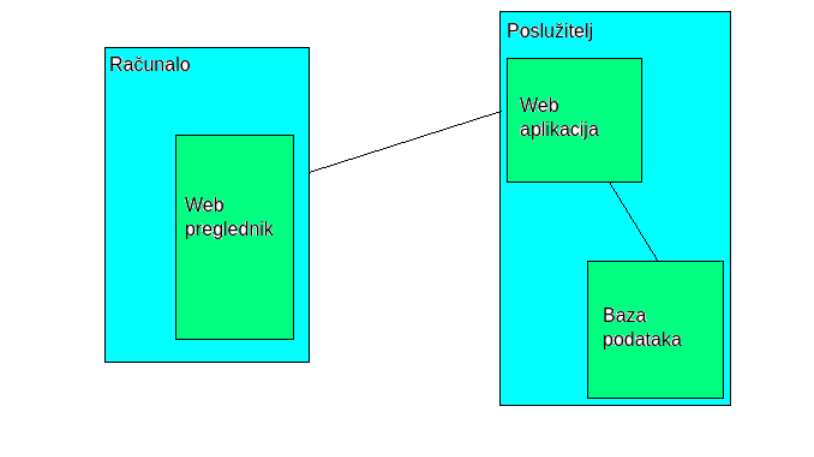
\includegraphics[width=\textwidth]{slike/arhitektura.png}
			\centering
			\caption{Arhitektura sustava}
			\label{fig:arhitektura_sustava}
		\end{figure}
	
		\underline{\textit{Web preglednik}} (eng. \textit{web browser}) je korisnički program koji omogućuje pregledavanje statičkih i dinamičkih sadržaja interneta. Web preglednik dohvaća sadržaj s lokalnog ili udaljenog računala, i potom taj sadržaj interpretira i prikazuje korisniku. Neki od popularnijih web preglednika današnjice su Chrome, Safari, Firefox i Edge.
		
		\underline{\textit{Web poslužitelj}} (eng. \textit{web server}) je temelj aplikacije, a služi za komunikaciju. Korisnik i aplikacija razmjenjuju HTTP zahtjeve (eng. \textit{HTTP request}) i HTTP odgovore (eng. \textit{HTTP response}). Poslužitelj pokreće prednji kraj (eng. \textit{front end}) i stražnji kraj (eng. \textit{back end}). Radi jednostavnosti, baza podataka je također smještena na poslužitelju.
		
		Korisnik kroz grafičko sučelje, odnosno prednji kraj, šalje zahtjeve na REST pristupne točke stražnjeg kraja. Tada stražnji kraj procesuira zahtjev i ako je potrebno komunicira s bazom podataka. Nakon konstrukcije, stražnji kraj šalje odgovor prednjem kraju u obliku JSON objekta, a prednji kraj procesuira odgovor i promjene prikazuje korisniku u obliku HTML stranice. 
		
		Za aplikaciju je odabrana višeslojna arhitektura temeljena na \textbf{MVC} (\textit{model-view-controller}) arhitekturnom stilu te uslužnoj arhitekturi.
		
		\begin{enumerate}
			\item \textit{sloj korisničke strane} - korisničko sučelje implementirano u JavaScriptu i radnom okviru AngularJS
			\item \textit{sloj nadglednika} - REST nadglednici 
			\item \textit{sloj domene} - model podataka iz domene primjene
			\item \textit{sloj za pristup podacima} - posrednik između sloja domene i baze podataka
			\item \textit{sloj baze podataka} - pohrana podataka
		\end{enumerate}
		
		Ovakva arhitektura odabrana je zbog poželjnih svojstava MVC arhitekturnog stila i višeslojne arhitekture: razvoj pojedinih slojeva jednostavniji je i u velikom stupnju nezavisan od razvoja drugih slojeva. Također, komunikacija prednjeg i stražnjeg kraja je ostvarena primjenom REST arhitketurnog stila. Zbog toga su prednji i stražnji kraj neovisni u smislu jezika implementacije, što potiče ponovnu uporabu.
		
		MVC arhitekturni stil sastoji se od tri koncepta:
		\begin{itemize}
			\item \textbf{Model} - reprezentacija strukture podataka koja se koristi u rješenju, neovisna o korisničkom sučeju
			\item \textbf{View} - pogled na podatke, u našoj aplikaciji to je grafičko sučelje
			\item \textbf{Controller} - nadzornik koji koordinira zahtjeve i odgovore između modela i pogleda, sadrži svu logiku upravljanja.
		\end{itemize}
				
		\section{Baza podataka}
			
			Za našu web aplikaciju koristimo PostgreSQL relacijsku bazu podataka. Pogodna je jer ima široku korisničku podršku, dokazanu stabilnost, dostupnost sučelja s Javom, a i već smo upoznati s njom iz prijašnjih iskustva. Relacijska baza podataka omogućuje jednostavno modeliranje problema domene, a temeljna joj je zadaća sigurna i brza pohrana i dohvat podataka. Temeljna građevna jedinica baze podataka je relacija, odnosno tablica. Jedna tablica predstavlja jedan entitet, a naša baza sastoji se od ovih relacija :
		
			\begin{itemize}
				\item user
				\item media
				\item pets
				\item posts
				\item comments
				\item relationships
				\item events
				\item event responses
				\item event comments
				\item company services
				\item company info
				\item messages
				\item reports
				\item blocks
			\end{itemize}
		
			\subsection{Opis tablica}
				
				\textbf{user} - Ovaj entitet predstavlja korisnika. Sadrži atribute ID, korisničko ime, lozinka, ime, prezime, email, tip korisnika, uloga korisnika, ID profilne slike.
				
				\begin{longtblr}[
					label=none,
					entry=none
					]{
						width = \textwidth,
						colspec={|X[8,l]|X[6, l]|X[20, l]|}, 
						rowhead = 1,
					} %definicija širine tablice, širine stupaca, poravnanje i broja redaka naslova tablice
					\hline \multicolumn{3}{|c|}{\textbf{user}}	 \\ \hline[3pt]
					\SetCell{LightGreen}id & SERIAL	& jedinstveni identifikator korisnika  	\\ \hline
					username & VARCHAR & korisničko ime  	\\ \hline 
					password & VARCHAR & korisnička lozinka \\ \hline 
					first\_name & VARCHAR & ime korisnika		\\ \hline 
					last\_name & VARCHAR & prezime korisnika		\\ \hline
					email & VARCHAR & korisnikov email			\\ \hline
					user\_type & ENUM & tip korisnika		\\ \hline
					user\_role & ENUM & uloga korisnika		\\ \hline
					\SetCell{LightBlue} profile\_picture\_id & BIGINT & id korisničke slike	\\ \hline
				\end{longtblr}
				
				\textbf{media} - Ovaj entitet predstavlja medijski sadržaj. Sadrži atribute ID i sam medijski sadržaj.
			
				\begin{longtblr}[
					label=none,
					entry=none
					]{
						width = \textwidth,
						colspec={|X[8,l]|X[6, l]|X[20, l]|}, 
						rowhead = 1,
					} %definicija širine tablice, širine stupaca, poravnanje i broja redaka naslova tablice
					\hline \multicolumn{3}{|c|}{\textbf{media}}	 \\ \hline[3pt]
					\SetCell{LightGreen}id & BIGSERIAL	& jedinstveni identifikator sadržaja   \\ \hline
					content & BYTEA & sadržaj  	\\ \hline 
				\end{longtblr}
				
				\textbf{pets} - Ovaj entitet predstavlja kućnog ljubimca. Sadrži atribute ID, tip ljubimca, ime, vlasnik, dob, spol, ID profilne slike, opis, pasmina.
				
				\begin{longtblr}[
					label=none,
					entry=none
					]{
						width = \textwidth,
						colspec={|X[8,l]|X[6, l]|X[20, l]|}, 
						rowhead = 1,
					} %definicija širine tablice, širine stupaca, poravnanje i broja redaka naslova tablice
					\hline \multicolumn{3}{|c|}{\textbf{pets}}	 \\ \hline[3pt]
					\SetCell{LightGreen}id & BIGSERIAL	& jedinstveni identifikator ljubimca  	\\ \hline
					type & ENUM & tip životinje  	\\ \hline 
					name & VARCHAR & ime ljubimca  	\\ \hline 
					age & INT & dob ljubimca		\\ \hline 
					gender & ENUM & spol ljubimca		\\ \hline
					description & VARCHAR & opis ljubimca		\\ \hline
					breed & VARCHAR & pasmina		\\ \hline
					\SetCell{LightBlue} owner & BIGINT & id vlasnika ljubimca \\ \hline 
					\SetCell{LightBlue} profile\_picture\_id & BIGINT & id korisničke slike	\\ \hline
				\end{longtblr}
			
				\textbf{posts} - Ovaj entitet predstavlja objavu. Sadrži atribute ID, ID korisnika, ID sadržaja i opis, odnosno samu objavu.
				
				\begin{longtblr}[
					label=none,
					entry=none
					]{
						width = \textwidth,
						colspec={|X[8,l]|X[6, l]|X[20, l]|}, 
						rowhead = 1,
					} %definicija širine tablice, širine stupaca, poravnanje i broja redaka naslova tablice
					\hline \multicolumn{3}{|c|}{\textbf{posts}}	 \\ \hline[3pt]
					\SetCell{LightGreen}id & BIGSERIAL	& jedinstveni identifikator objave 	\\ \hline
					\SetCell{LightBlue} user\_id & BIGINT & id korisnika koji objavljuje 	\\ \hline 
					\SetCell{LightBlue} content\_id & BIGINT & id medijskog sadržaja \\ \hline 
					description & VARCHAR & sadržaj objave		\\ \hline 
				\end{longtblr}
			
				\textbf{comments} - Ovaj entitet predstavlja komentar na objavu. Sadrži atribute ID, ID korisnika, ID objave i sadržaj, odnosno komentar.
				
				\begin{longtblr}[
					label=none,
					entry=none
					]{
						width = \textwidth,
						colspec={|X[8,l]|X[6, l]|X[20, l]|}, 
						rowhead = 1,
					} %definicija širine tablice, širine stupaca, poravnanje i broja redaka naslova tablice
					\hline \multicolumn{3}{|c|}{\textbf{comments}}	 \\ \hline[3pt]
					\SetCell{LightGreen}id & BIGSERIAL	& jedinstveni identifikator objave 	\\ \hline
					\SetCell{LightBlue} user\_id & BIGINT & id korisnika koji objavljuje komentar 	\\ \hline 
					\SetCell{LightBlue} post\_id & BIGINT & id objave na koju se komentira \\ \hline 
					content & VARCHAR & sadržaj komentara		\\ \hline 
				\end{longtblr}
			
				\textbf{relationships} - Ovaj entitet predstavlja odnose između dva korisnika. Sadrži atribute prvi korisnik, drugi korisnik, tip odnosa između njih.
				
				\begin{longtblr}[
					label=none,
					entry=none
					]{
						width = \textwidth,
						colspec={|X[8,l]|X[6, l]|X[20, l]|}, 
						rowhead = 1,
					} %definicija širine tablice, širine stupaca, poravnanje i broja redaka naslova tablice
					\hline \multicolumn{3}{|c|}{\textbf{relationships}}	 \\ \hline[3pt]
					\SetCell{LightBlue} first\_user & BIGINT & id prvog korisnika		\\ \hline 
					\SetCell{LightBlue} second\_user & BIGINT & id drugog korisnika		\\ \hline
					type & ENUM & tip odnosa između dva korisnika		\\ \hline
				\end{longtblr}
			
				\textbf{events} - Ovaj entitet predstavlja događaje. Sadrži atribute id, organizator, početak, trajanje, opis, lokacija, vidljivost.
				
				\begin{longtblr}[
					label=none,
					entry=none
					]{
						width = \textwidth,
						colspec={|X[8,l]|X[6, l]|X[20, l]|}, 
						rowhead = 1,
					} %definicija širine tablice, širine stupaca, poravnanje i broja redaka naslova tablice
					\hline \multicolumn{3}{|c|}{\textbf{events}}	 \\ \hline[3pt]
					\SetCell{LightGreen}id & BIGSERIAL	& jedinstveni identifikator događaja  	\\ \hline
					\SetCell{LightBlue} organizer & BIGINT & id korisnika organizatora  	\\ \hline 
					start\_date & TIMESTAMP & vrijeme i datum početka događaja	\\ \hline 
					duration & INTERVAL & trajanje događaja \\ \hline 
					description & VARCHAR & opis događaja		\\ \hline
					location & VARCHAR & lokacija događaja			\\ \hline
					visibility & ENUM & vidljivost događaja		\\ \hline
				\end{longtblr}
			
				\textbf{event\_responses} - Ovaj entitet predstavlja odgovore na događaje. Sadrži atribute ID događaja, ID korisnika, odgovor na događaj.
				
				\begin{longtblr}[
					label=none,
					entry=none
					]{
						width = \textwidth,
						colspec={|X[8,l]|X[6, l]|X[20, l]|}, 
						rowhead = 1,
					} %definicija širine tablice, širine stupaca, poravnanje i broja redaka naslova tablice
					\hline \multicolumn{3}{|c|}{\textbf{event\_responses}}	 \\ \hline[3pt]
					\SetCell{LightBlue}event\_id & BIGINT & id događaja 		\\ \hline
					\SetCell{LightBlue}user\_id & BIGINT & id korisnika		\\ \hline
					response & ENUM & odgovor o dolasku	\\ \hline
				\end{longtblr}
				
				\textbf{event\_comments} - Ovaj entitet predstavlja komentare na događaj. Sadrži atribute ID, ID događaja, ID korisnika, komentar.
				
				\begin{longtblr}[
					label=none,
					entry=none
					]{
						width = \textwidth,
						colspec={|X[8,l]|X[6, l]|X[20, l]|}, 
						rowhead = 1,
					} %definicija širine tablice, širine stupaca, poravnanje i broja redaka naslova tablice
					\hline \multicolumn{3}{|c|}{\textbf{event\_comments}}	 \\ \hline[3pt]
					\SetCell{LightGreen} id & BIGSERIAL & jedinstveni identifikator komentara	\\ \hline
					\SetCell{LightBlue}event\_id & BIGINT & id događaja 		\\ \hline
					\SetCell{LightBlue}user\_id & BIGINT & id korisnika		\\ \hline
					content & VARCHAR & sadržaj komentara	\\ \hline
				\end{longtblr}
			
				\textbf{company\_services} - Ovaj entitet predstavlja uslugu koju pruža neka tvrtka. Sadrži atribute ID tvrtke, tip usluge, opis usluge.
				
				\begin{longtblr}[
					label=none,
					entry=none
					]{
						width = \textwidth,
						colspec={|X[8,l]|X[6, l]|X[20, l]|}, 
						rowhead = 1,
					} %definicija širine tablice, širine stupaca, poravnanje i broja redaka naslova tablice
					\hline \multicolumn{3}{|c|}{\textbf{company\_services}}	 \\ \hline[3pt]
					\SetCell{LightBlue}company\_id & BIGINT & jedinstveni identifikator tvrtke	\\ \hline
					service\_type & ENUM & vrsta usluge 		\\ \hline
					service\_description & VARCHAR & opis usluge		\\ \hline
				\end{longtblr}
			
				\textbf{company\_info} - Ovaj entitet predstavlja opis tvrtke. Sadrži atribute ID tvrtke, ime, adresa, kontakt.
				
				\begin{longtblr}[
					label=none,
					entry=none
					]{
						width = \textwidth,
						colspec={|X[8,l]|X[6, l]|X[20, l]|}, 
						rowhead = 1,
					} %definicija širine tablice, širine stupaca, poravnanje i broja redaka naslova tablice
					\hline \multicolumn{3}{|c|}{\textbf{company\_info}}	 \\ \hline[3pt]
					\SetCell{LightBlue}company\_id & BIGINT & jedinstveni identifikator tvrtke		\\ \hline
					name & VARCHAR & ime tvrtke		\\ \hline
					adress & VARCHAR & adresa tvrtke		\\ \hline
					contact & VARCHAR & kontakt tvrtke		\\ \hline
				\end{longtblr}
			
				\textbf{messages} - Ovaj entitet predstavlja poruke između korisnika. Sadrži atribute ID, pošiljatelj, primatelj, sadržaj.
				
				\begin{longtblr}[
					label=none,
					entry=none
					]{
						width = \textwidth,
						colspec={|X[8,l]|X[6, l]|X[20, l]|}, 
						rowhead = 1,
					} %definicija širine tablice, širine stupaca, poravnanje i broja redaka naslova tablice
					\hline \multicolumn{3}{|c|}{\textbf{messages}}	 \\ \hline[3pt]
					\SetCell{LightGreen} id & BIGSERIAL & id događaja 		\\ \hline
					\SetCell{LightBlue}sender & BIGINT & id pošiljatelja		\\ \hline
					\SetCell{LightBlue}receiver & BIGINT & id primatelja		\\ \hline
					content & VARCHAR & sadržaj poruke	\\ \hline
				\end{longtblr}
				
				\textbf{reports} - Ovaj entitet predstavlja prijavu nekog korisnika. Sadrži atribute ID korisnika koji prijavljuje, ID korisnika koji je prijavljen, opis, ID objave, ID poruke, ID komentara.
				
				\begin{longtblr}[
					label=none,
					entry=none
					]{
						width = \textwidth,
						colspec={|X[8,l]|X[6, l]|X[20, l]|}, 
						rowhead = 1,
					} %definicija širine tablice, širine stupaca, poravnanje i broja redaka naslova tablice
					\hline \multicolumn{3}{|c|}{\textbf{reports}}	 \\ \hline[3pt]
					\SetCell{LightBlue}reporter\_id & BIGINT & id korisnika koji prijavljuje		\\ \hline
					\SetCell{LightBlue}reported\_user & BIGINT & id korisnika koji je prijavljen		\\ \hline
					description & VARCHAR & opis prijave	\\ \hline
					\SetCell{LightBlue}post\_id & BIGINT & id objave		\\ \hline
					\SetCell{LightBlue}message\_id & BIGINT & id poruke		\\ \hline
					\SetCell{LightBlue}comment\_id & BIGINT & id komentara	\\ \hline	
				\end{longtblr}
			
				\textbf{blocks} - Ovaj entitet predstavlja blokiranje korisnika. Sadrži atribute ID korisnika, datum odblokiranja.
				
				\begin{longtblr}[
					label=none,
					entry=none
					]{
						width = \textwidth,
						colspec={|X[8,l]|X[6, l]|X[20, l]|}, 
						rowhead = 1,
					} %definicija širine tablice, širine stupaca, poravnanje i broja redaka naslova tablice
					\hline \multicolumn{3}{|c|}{\textbf{blocks}}	 \\ \hline[3pt]
					\SetCell{LightBlue}user\_id & BIGINT & id korisnika		\\ \hline
					end\_time & TIMESTAMP & vrijeme prestanka blokiranja		\\ \hline
				\end{longtblr}
			
			\subsection{Dijagram baze podataka}
				\begin{figure}[H]
					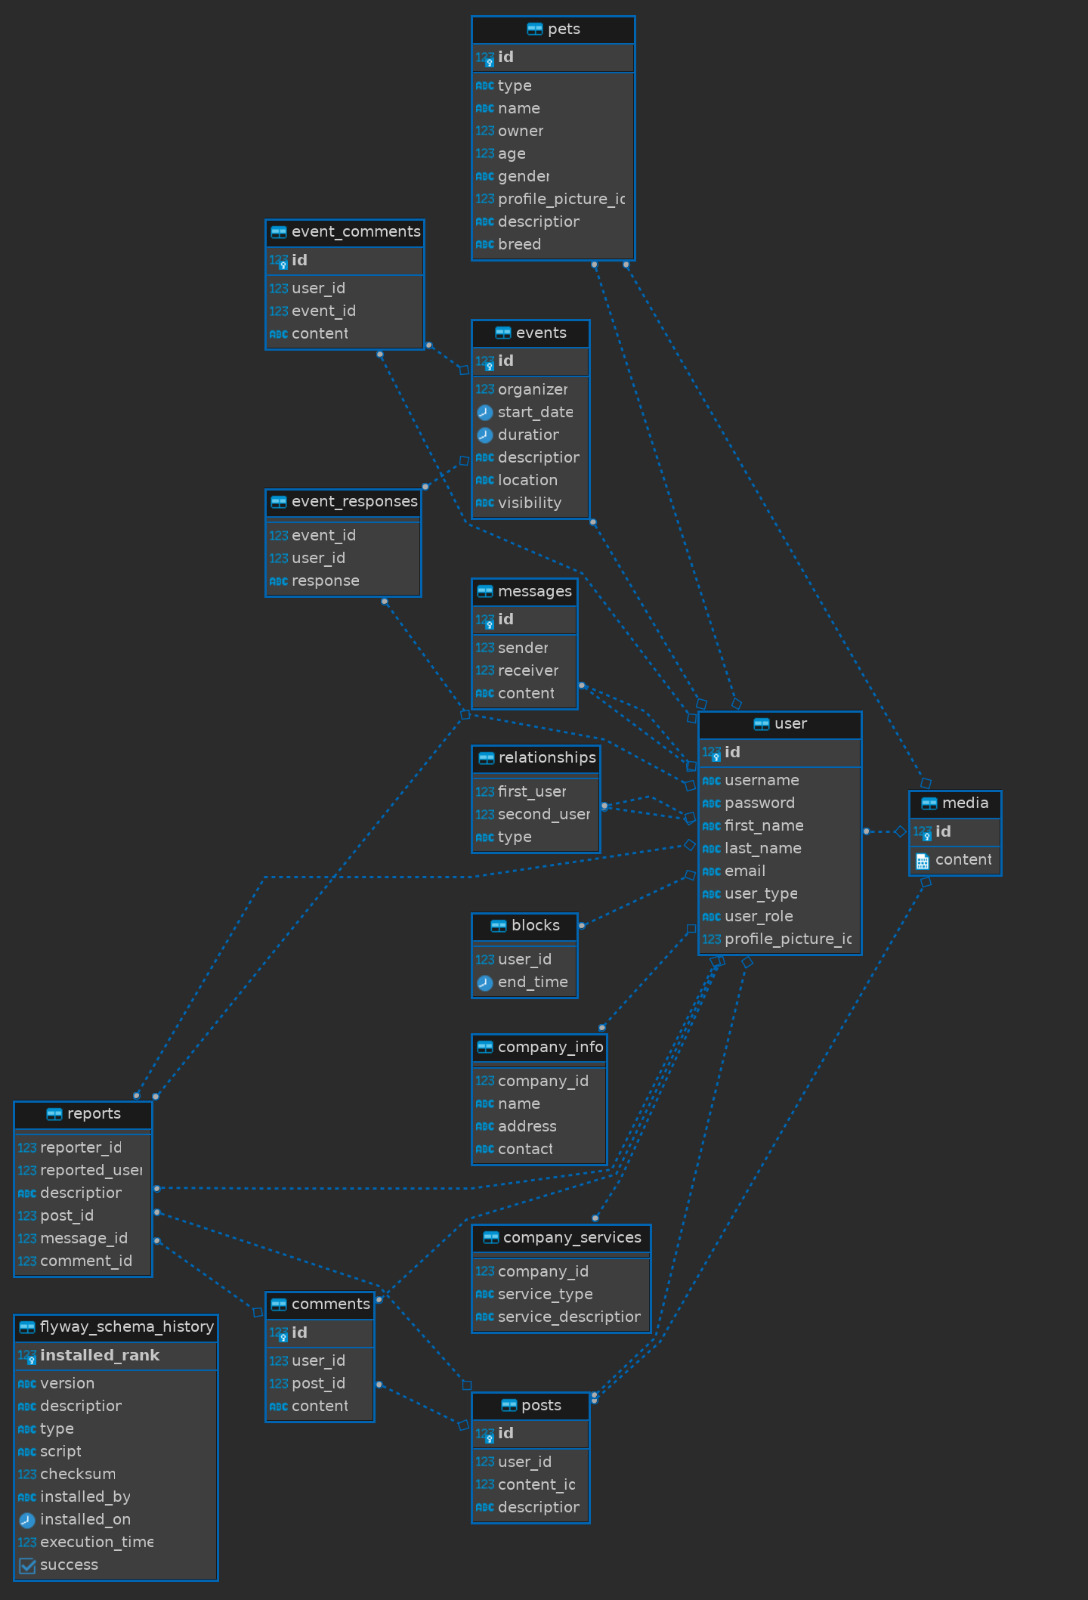
\includegraphics[scale = 0.37]{slike/dijagram_baze.jpeg}
					\centering
					\caption{Dijagram baze podataka}
					\label{fig:dijagram_baze}
				\end{figure}
			
			\eject
			
			
		\section{Dijagram razreda}
		
			Dijagram razreda prikazuje odnose izmedu različitih objekata, te njihove atribute
			i operacije kojima vladaju. Radi jednostavnosti, dijagram razreda je
			podijeljen u više slika.
			
			\begin{figure}[H]
				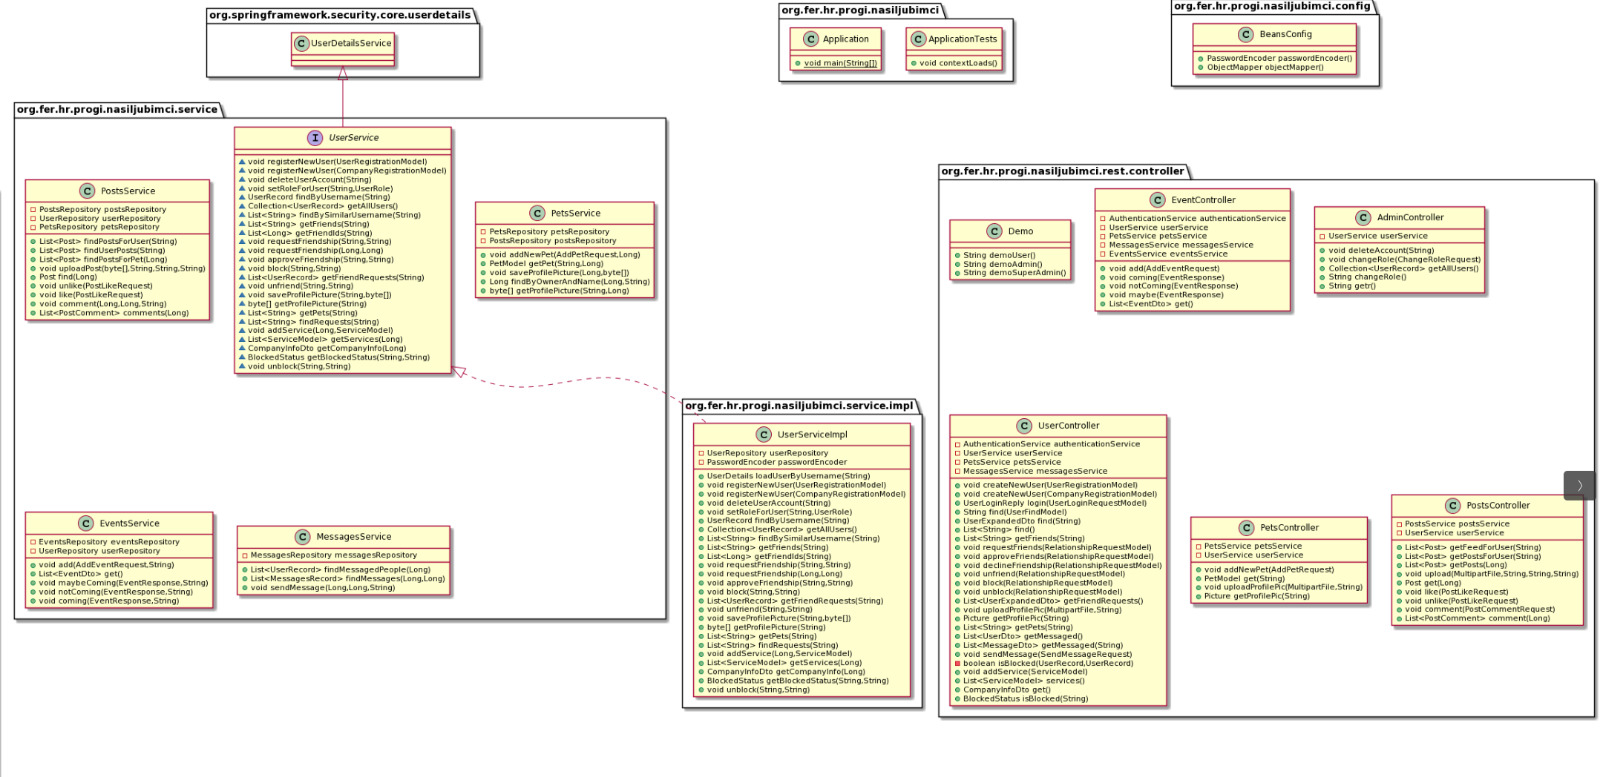
\includegraphics[scale=0.3]{slike/controller.jpeg} %veličina slike u odnosu na originalnu datoteku i pozicija slike
				\centering
				\caption{Dijagram razreda kontrolera}
			\end{figure}
		
			\begin{figure}[H]
				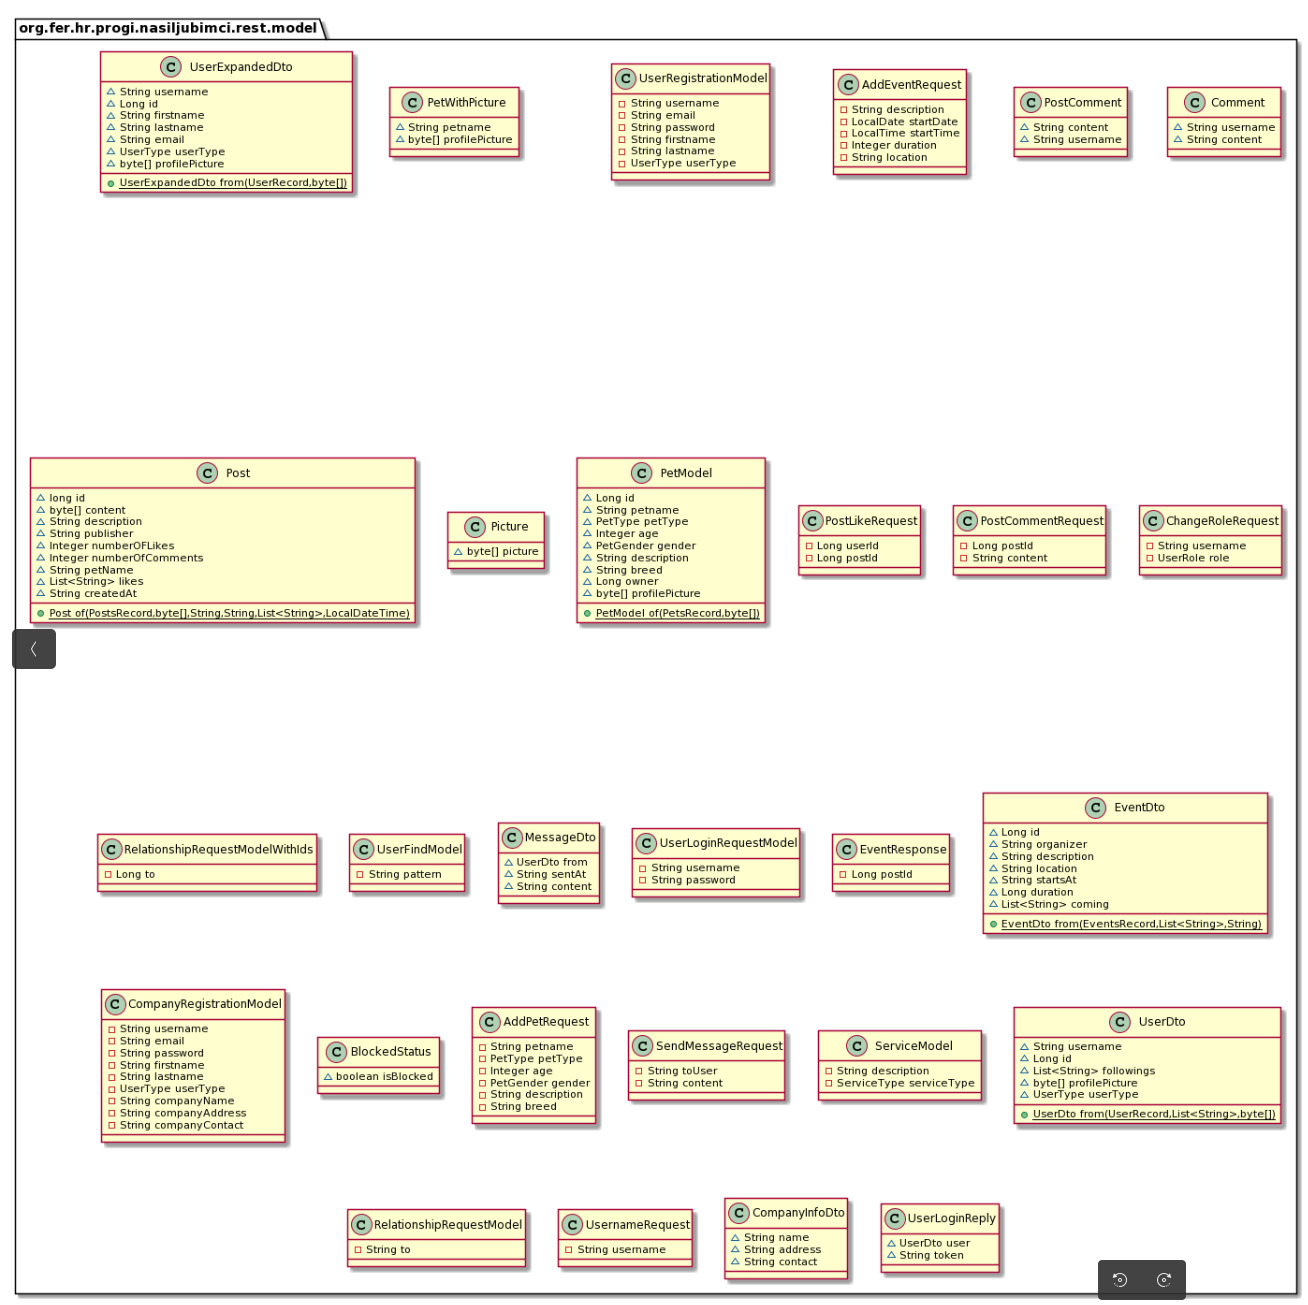
\includegraphics[scale=0.34]{slike/rest_model.jpeg} %veličina slike u odnosu na originalnu datoteku i pozicija slike
				\centering
				\caption{Dijagram razreda rest modela}
			\end{figure}
		
			\begin{figure}[H]
				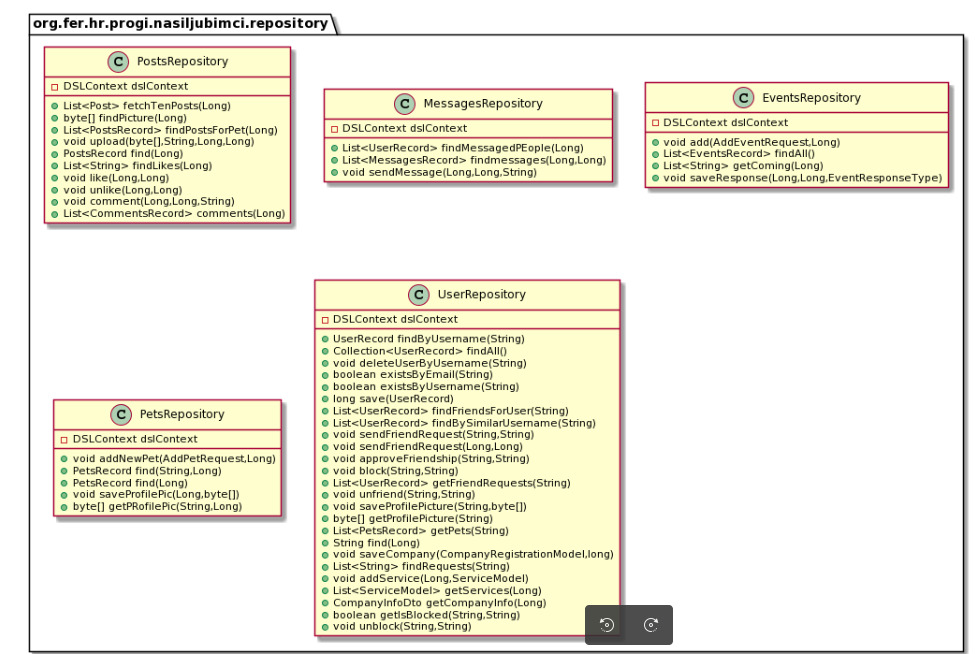
\includegraphics[scale=0.4]{slike/repository.jpeg} %veličina slike u odnosu na originalnu datoteku i pozicija slike
				\centering
				\caption{Dijagram razreda repozitorija}
			\end{figure}
		
			\begin{figure}[H]
				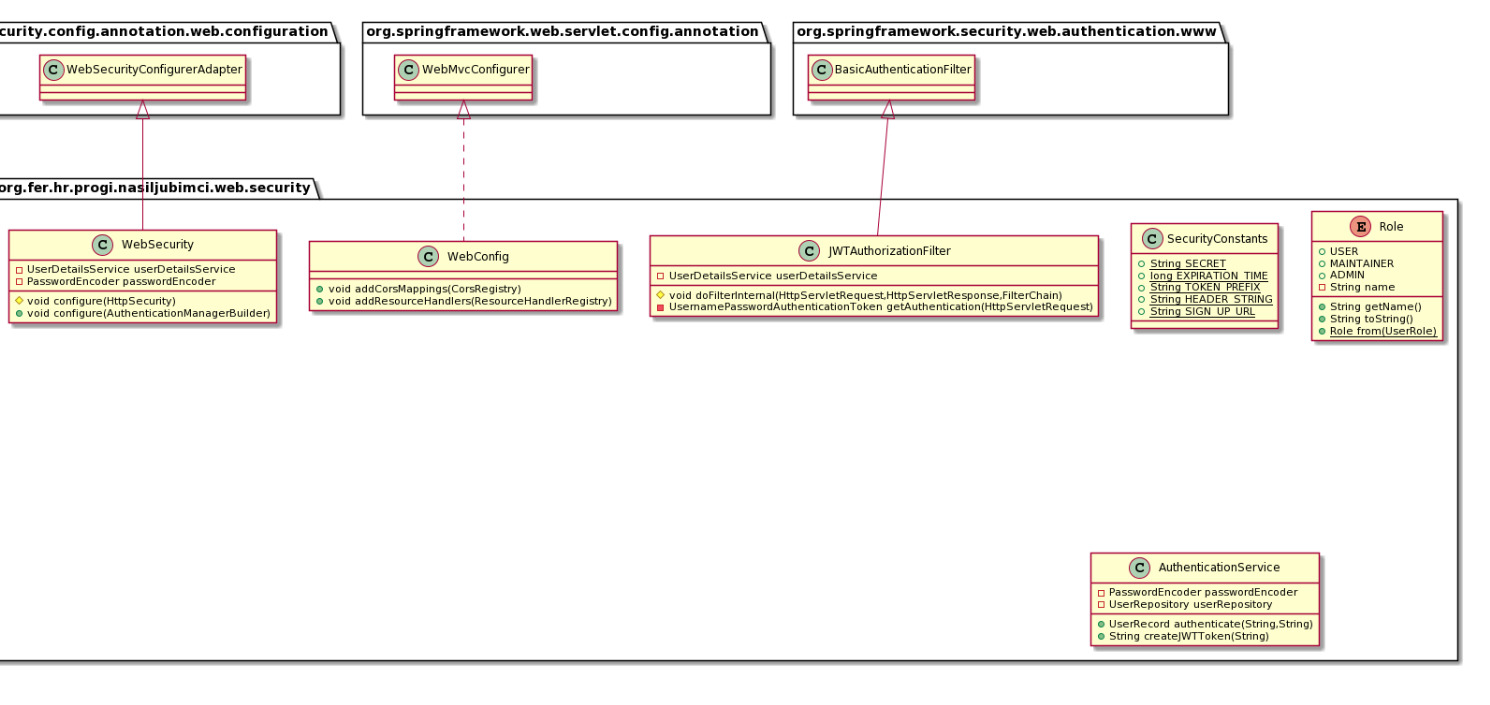
\includegraphics[scale=0.3]{slike/security.jpeg} %veličina slike u odnosu na originalnu datoteku i pozicija slike
				\centering
				\caption{Dijagram razreda securityja}
			\end{figure}
			
			
			\eject
		
		\section{Dijagram stanja}
			
			Dijagram stanja primjenjuje se za opis stanja objekta i za opisivanje prijelaza iz jednog u drugo stanje. Priložena slika prikazuje dijagram stanja objekta "Vlasnik". Vlasnik se prijavljuje u aplikaciju te nakon toga on prelazi u stanje "Početna stranica". S "Početne stranice" može prijeći na svoj "Osobni profil" odakle može izvršiti niz akcija. U završno stanje dolazi se nakon stanja "Početna stranica" i odjave iz aplikacije.
			\begin{figure}[H]
				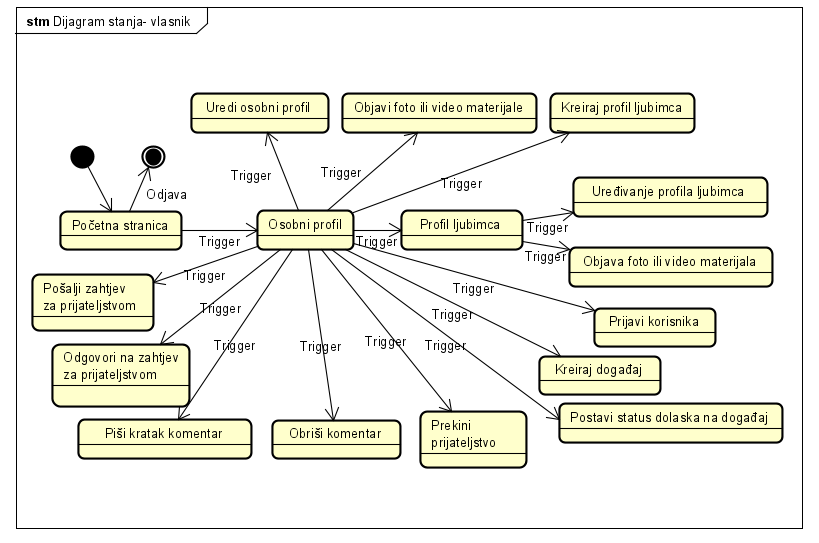
\includegraphics[width=\textwidth]{slike/Dijagram_stanja_vlasnik.png}
				\centering
				\caption{Dijagram stanja}
				\label{fig:classd_middle}
			\end{figure}
			
			
			\eject 
		
		\section{Dijagram aktivnosti}
			
			Dijagram aktivnosti prikazuje povezane aktivnosti na visokoj apstrakcijskoj razini. Dijagram aktivnosti intuitivno prikazuje kako podaci teku kroz aplikaciju i kako se kontrola nad podacima mijenja. Idući dijagram prikazuje proces prijave korisnika na neki od nadolazećih događaja.
			
			\begin{figure}[H]
				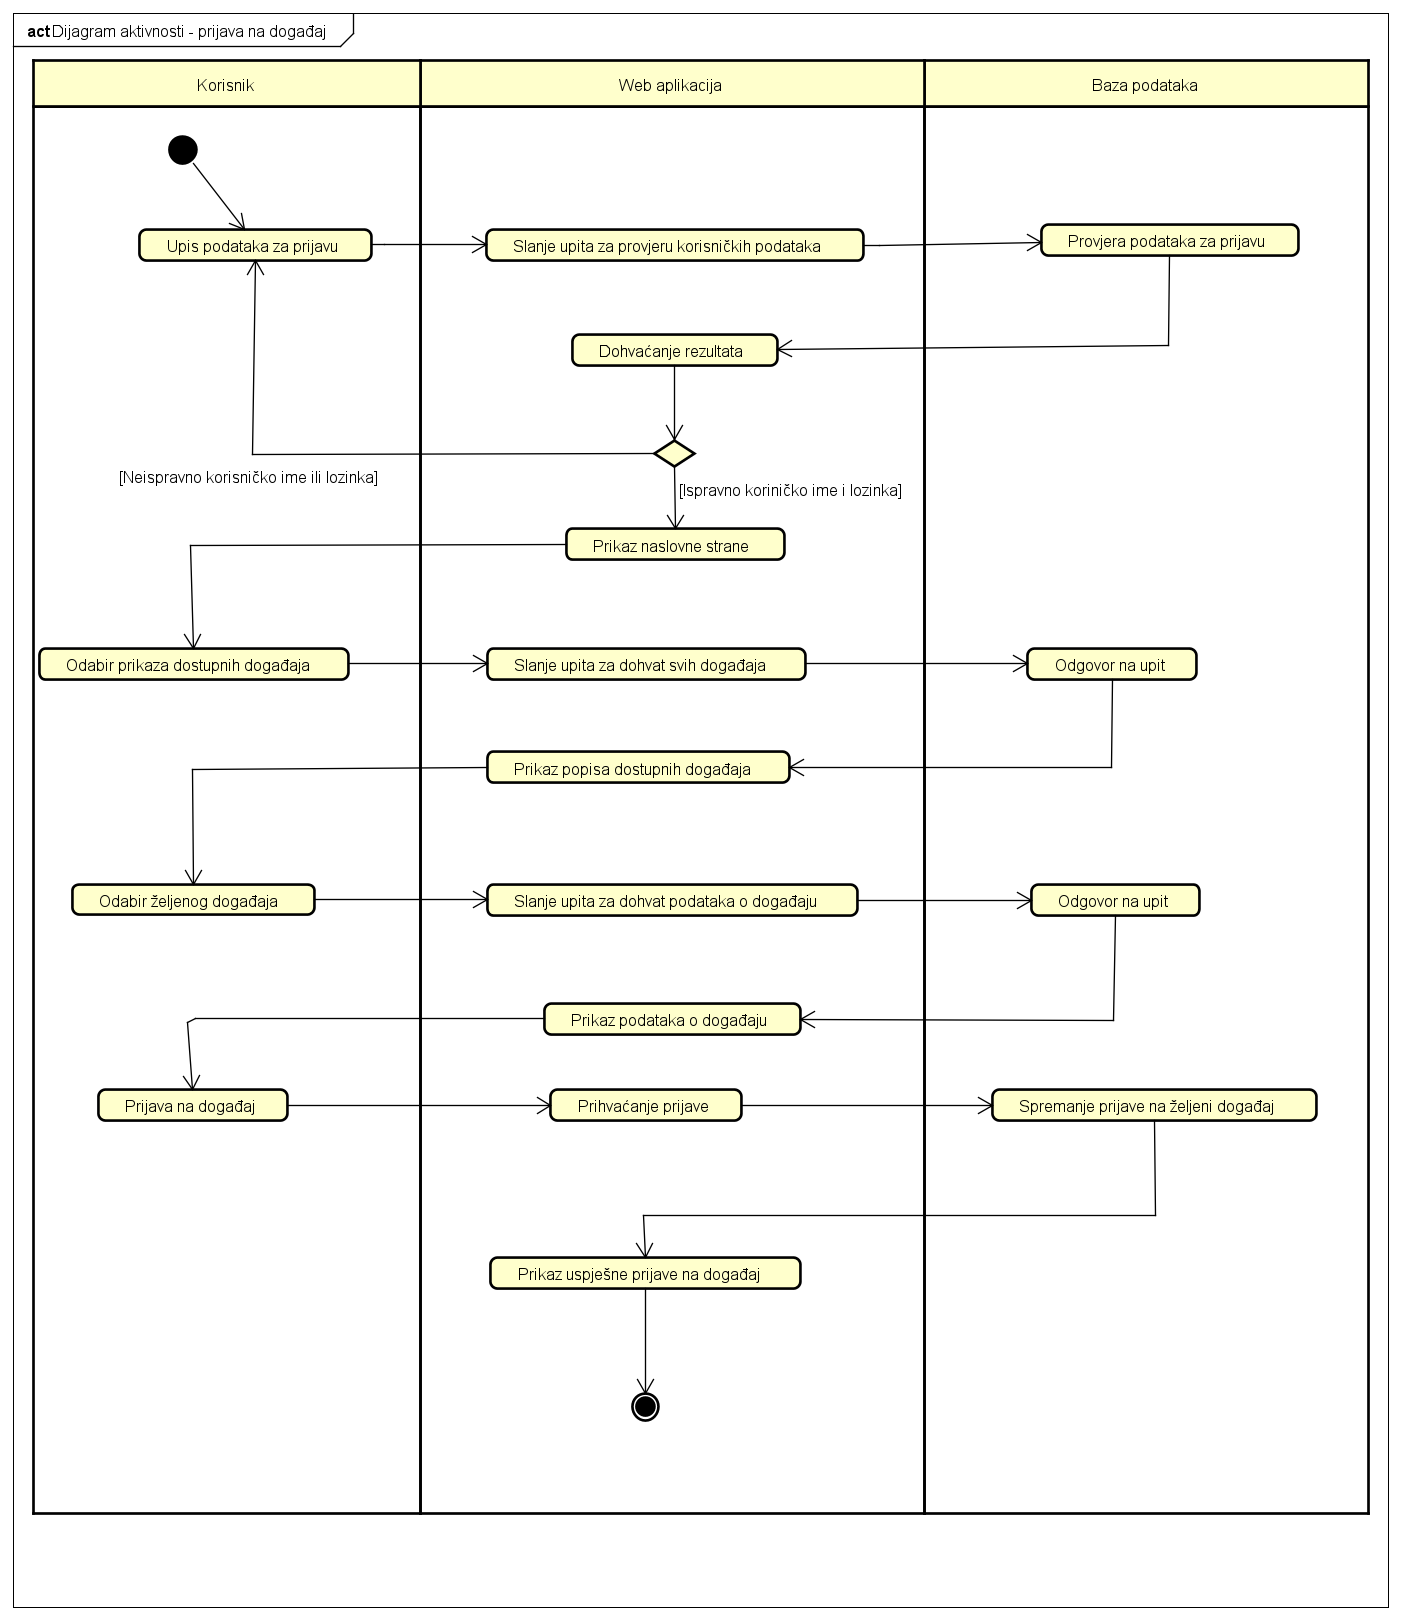
\includegraphics[width=\textwidth]{slike/Dijagram_aktivnosti.png}
				\centering
				\caption{Dijagram aktivnosti}
				\label{fig:classd_middle}
			\end{figure}
			
			\eject
		\section{Dijagram komponenti}
		
			\textbf{\textit{dio 2. revizije}}\\
		
			 \textit{Potrebno je priložiti dijagram komponenti s pripadajućim opisom. Dijagram komponenti treba prikazivati strukturu cijele aplikacije.}
	\chapter{Implementacija i korisničko sučelje}
		
		
		\section{Korištene tehnologije i alati}
		
			Komunikacija u timu realizirana je putem mobilne aplikacije  \underline{WhatsApp}\footnote{\url{https://www.whatsapp.com}}. 
			Za izradu UML dijagrama korišten je alat \underline{Astah Professional}\footnote{\url{https://astah.net/products/astah-professional/}}, a kao sustav za upravljanje izvornim kodom \underline{Git}\footnote{\url{https://git-scm.com/}}. 
			Udaljeni repozitorij projekta je dostupan na web platformi \underline{GitLab}\footnote{\url{https://gitlab.com/}}.
			\par
			Kao razvojno okruženje korišten je \underline{Eclipse}\footnote{\url{https://www.eclipse.org/}} - integrirano razvojno okruženje. Eclipse je većinom pisan u Javi i prvenstveno se koristi za razvoj Java aplikacija, ali koristi se i za razvoj aplikacija u drugim programskim jezicima kao što su C, C++, PHP, Python i još mnogi drugi.
			\par
			Za razvoj korisničkog sučelja i frontenda korišten je uređivač teksta \underline{VSCode}\footnote{\url{https://code.visualstudio.com/}}. Taj uređivač teksta je danas jedan od najrasprostranjenijih i koristi se u svim sferama industrije. 
			\par
			Aplikacija je napisana u \underline{Javi}\footnote{\url{https://www.java.com/en/}} koristeći ekosustav \underline{Java Spring}\footnote{\url{https://spring.io/}} za
			izradu backenda te \underline{React}\footnote{\url{https://reactjs.org/}} i \underline{JavaScript}\footnote{\url{https://www.javascript.com/}} za izradu frontenda. 
			\par
			Za bazu podataka koristili smo (\underline{PostgreSQL}\footnote{\url{https://www.postgresql.org/}}).
			
			
			\eject 
		
	
		\section{Ispitivanje programskog rješenja}
			
			\textbf{\textit{dio 2. revizije}}\\
			
			 \textit{U ovom poglavlju je potrebno opisati provedbu ispitivanja implementiranih funkcionalnosti na razini komponenti i na razini cijelog sustava s prikazom odabranih ispitnih slučajeva. Studenti trebaju ispitati temeljnu funkcionalnost i rubne uvjete.}
	
			
			\subsection{Ispitivanje komponenti}
			\textit{Potrebno je provesti ispitivanje jedinica (engl. unit testing) nad razredima koji implementiraju temeljne funkcionalnosti. Razraditi \textbf{minimalno 6 ispitnih slučajeva} u kojima će se ispitati redovni slučajevi, rubni uvjeti te izazivanje pogreške (engl. exception throwing). Poželjno je stvoriti i ispitni slučaj koji koristi funkcionalnosti koje nisu implementirane. Potrebno je priložiti izvorni kôd svih ispitnih slučajeva te prikaz rezultata izvođenja ispita u razvojnom okruženju (prolaz/pad ispita). }
			
			
			
			\subsection{Ispitivanje sustava}
			
			 \textit{Potrebno je provesti i opisati ispitivanje sustava koristeći radni okvir Selenium\footnote{\url{https://www.seleniumhq.org/}}. Razraditi \textbf{minimalno 4 ispitna slučaja} u kojima će se ispitati redovni slučajevi, rubni uvjeti te poziv funkcionalnosti koja nije implementirana/izaziva pogrešku kako bi se vidjelo na koji način sustav reagira kada nešto nije u potpunosti ostvareno. Ispitni slučaj se treba sastojati od ulaza (npr. korisničko ime i lozinka), očekivanog izlaza ili rezultata, koraka ispitivanja i dobivenog izlaza ili rezultata.\\ }
			 
			 \textit{Izradu ispitnih slučajeva pomoću radnog okvira Selenium moguće je provesti pomoću jednog od sljedeća dva alata:}
			 \begin{itemize}
			 	\item \textit{dodatak za preglednik \textbf{Selenium IDE} - snimanje korisnikovih akcija radi automatskog ponavljanja ispita	}
			 	\item \textit{\textbf{Selenium WebDriver} - podrška za pisanje ispita u jezicima Java, C\#, PHP koristeći posebno programsko sučelje.}
			 \end{itemize}
		 	\textit{Detalji o korištenju alata Selenium bit će prikazani na posebnom predavanju tijekom semestra.}
			
			\eject 
		
		
		\section{Dijagram razmještaja}
			
			Dijagrami razmještaja prikazuju topologiju sustava i odnos sklopovskih i programskih dijelova. Olakšavaju nam vizualizaciju razmještaja fizičkog dijela sustava i sklopovlja. Sustav se sastoji od korisničkog i poslužiteljskog računala. Korisnik na svojem računalu preko web preglednika pristupa aplikaciji. Korisničko računalo komunicira s poslužiteljskim računalom preko HTTP veze. Na poslužiteljskom se računalu nalaze Web poslužitelj i poslužitelj baze podataka. 
			
			\begin{figure}[H]
				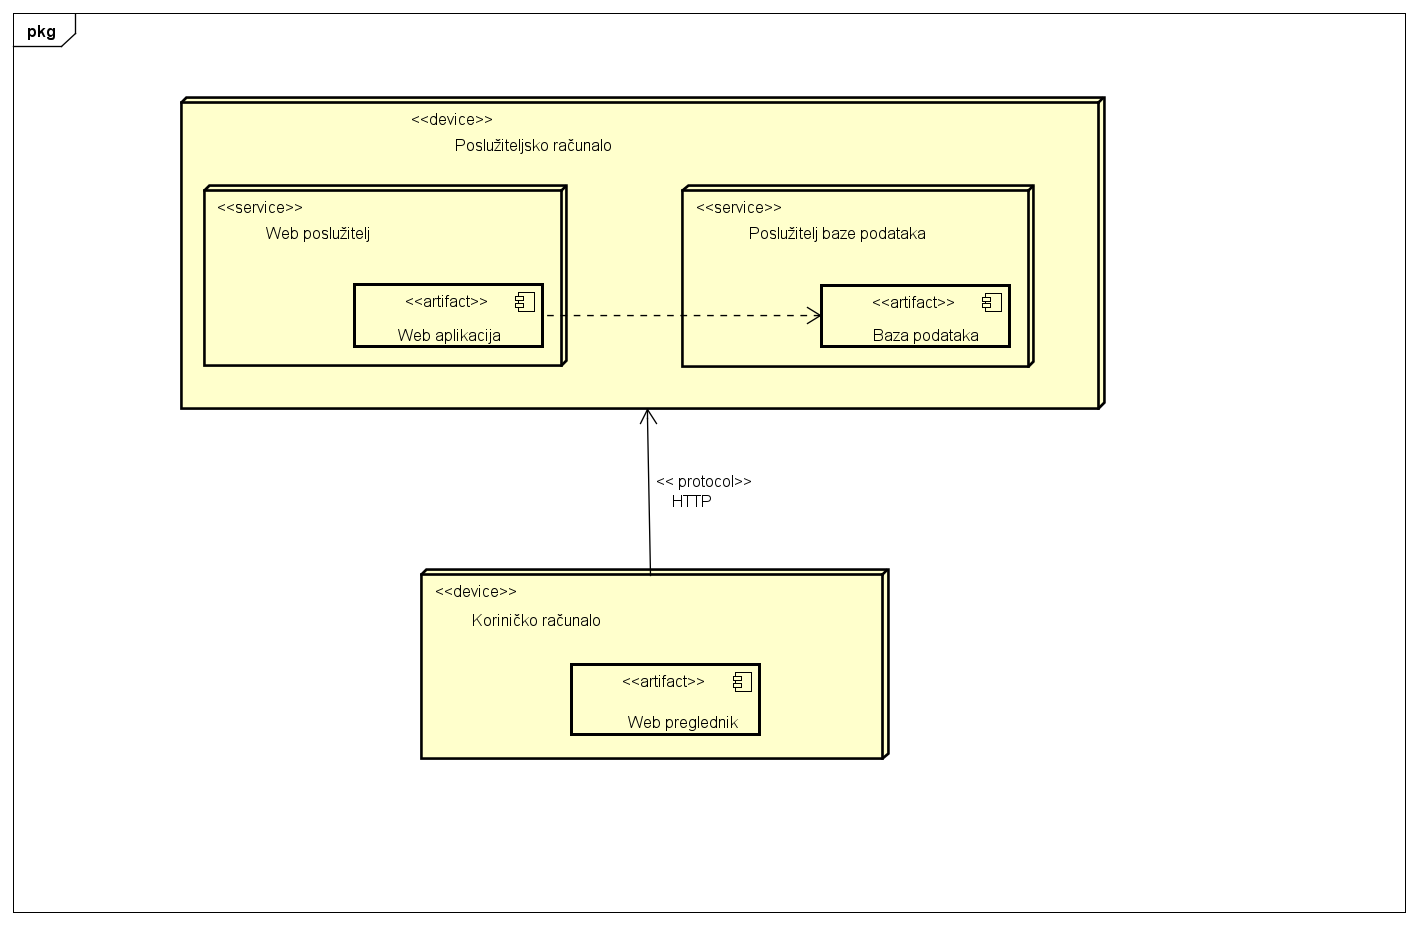
\includegraphics[width=\textwidth]{slike/Dijagram_razmjestaja.png}
				\centering
				\caption{Dijagram razmještaja}
				\label{fig:dijagram_razmjestaja}
			\end{figure}
			
			\eject 
		
		\section{Upute za puštanje u pogon}
		
			\textbf{\textit{dio 2. revizije}}\\
		
			 \textit{U ovom poglavlju potrebno je dati upute za puštanje u pogon (engl. deployment) ostvarene aplikacije. Na primjer, za web aplikacije, opisati postupak kojim se od izvornog kôda dolazi do potpuno postavljene baze podataka i poslužitelja koji odgovara na upite korisnika. Za mobilnu aplikaciju, postupak kojim se aplikacija izgradi, te postavi na neku od trgovina. Za stolnu (engl. desktop) aplikaciju, postupak kojim se aplikacija instalira na računalo. Ukoliko mobilne i stolne aplikacije komuniciraju s poslužiteljem i/ili bazom podataka, opisati i postupak njihovog postavljanja. Pri izradi uputa preporučuje se \textbf{naglasiti korake instalacije uporabom natuknica} te koristiti što je više moguće \textbf{slike ekrana} (engl. screenshots) kako bi upute bile jasne i jednostavne za slijediti.}
			
			
			 \textit{Dovršenu aplikaciju potrebno je pokrenuti na javno dostupnom poslužitelju. Studentima se preporuča korištenje neke od sljedećih besplatnih usluga: \href{https://aws.amazon.com/}{Amazon AWS}, \href{https://azure.microsoft.com/en-us/}{Microsoft Azure} ili \href{https://www.heroku.com/}{Heroku}. Mobilne aplikacije trebaju biti objavljene na F-Droid, Google Play ili Amazon App trgovini.}
			
			
			\eject 
	\chapter{Zaključak i budući rad}
		
		Naš zadatak bio je izraditi platformu koja bi vlasnicima kućnih ljubimaca omogućila druženje i komunikaciju s drugim vlasnicima, objavljivanje raznih medijskih sadržaja i pronalazak željenih usluga za njihove ljubimce.
		
		Projekt smo proveli u tri faze:
		\begin{enumerate}
			\item početna razrada funkcionalnih i nefunkcionalnih zahtjeva
			\item implementacija zahtjeva i daljnje razrađivanje
			\item testiranje i završno dokumentiranje
		\end{enumerate} 
	
		U prvoj fazi projekta proučavali smo funkcionalne zahtjeve aplikacije, odnosno što sve korisnici u njoj mogu obavljati. Ova faza bila je dosta teška u početku budući da se kao članovi tima nismo od prije poznavali, pa tako nismo ni previše znali koliko je tko iskusan u kojem području. Također, shvatili smo kako je prije izrade samog projekta potrebno vrlo dobro proučiti alate koje ćemo koristiti. 
		
		U drugoj fazi projekta krenuli smo s implementacijom koja nam je opet bila dosta teška budući da se nismo toliko dobro poznavali. No ipak smo s vremenom počeli implementirati zahtjeve sve lakše. Također, tijekom implementacije smo prepoznali propuste u definicijama funkcionalnih i nefunkcionalnih zahtjeva pa smo ih ponovno i preciznije definirali. 
		
		U trećoj smo fazi, nakon implementacije, dovršili i dokumentaciju projekta i obavili testiranje sustava. Tijekom pisanja dokumentacije smo prepoznali veličinu našeg projekta i vrijeme i organiziranost potrebno u izradi “pravih” projekata. 
		
		Članovi tima su prije projekta bili upoznati s Javom, Reactom i PostgreSQL-om pa smo tako i odabrali tehnologije koje smo koristili. 
		
		Naučili smo važnost dobre koordinacije i komunikacije s članovima tima. Također, naučili smo neke vještine povezane s projektima općenito, poput korištenja alata git i GitLab-a, te izrade dijagrama alatom Astah Professional.
		
		Najveću važnost tijekom projekta možemo pridodati vremenskoj organiziranosti. Ovakvi projekti su vremenski zahtjevni te je potrebna dobra usklađenost da nebi došlo do situacije u kojoj jedna implementacija ovisi o drugoj koja još nije dovršena. Budući da nismo radili na previše ovakvih projekata imali smo i takvih slučajeva, no uspješno smo ih riješili. 
		
		Od definiranih funkcionalnih zahtjeva, implementirali smo prijavu i registraciju korisnika, stvaranje i uređivanje profila ljubimca i korisnika, objavu medijskog sadržaja, komentiranje, slanje zahtjeva za prijateljstvo, stvaranje događaja, slanje poruka, prijava drugih korisnika, blokiranje i brisanje korisnika od strane administratora.  
		
		Tijekom testiranja smo uvidjeli da od početka treba biti temeljit i detaljan pri definiraju slučajeva korištenja i prepoznati rubne slučajeve. 
		
		Zaključno, stekli smo nova iskustva, znanja i susreli se s nekim novim alatima, no najvažnije je da smo dobili dojam kako je to raditi u timu na projektu koji zahtjeva izrazitu vremensku organiziranost i znanje da bi se dobro napravio. Vjerujem da bi projekt, ukoliko počinjemo ispočetka, napravili bolje i brže. 
		
		\eject 
	\chapter*{Popis literature}
		\addcontentsline{toc}{chapter}{Popis literature}
	 	
 		\textbf{\textit{Kontinuirano osvježavanje}}
	
		\textit{Popisati sve reference i literaturu koja je pomogla pri ostvarivanju projekta.}
		
		
		\begin{enumerate}
			
			
			\item  Programsko inženjerstvo, FER ZEMRIS, \url{http://www.fer.hr/predmet/proinz}
			
			\item  I. Sommerville, "Software engineering", 8th ed, Addison Wesley, 2007.
			
			\item  T.C.Lethbridge, R.Langaniere, "Object-Oriented Software Engineering", 2nd ed. McGraw-Hill, 2005.
			
			\item  I. Marsic, Software engineering book``, Department of Electrical and Computer Engineering, Rutgers University, \url{http://www.ece.rutgers.edu/~marsic/books/SE}
			
			\item  The Unified Modeling Language, \url{https://www.uml-diagrams.org/}
			
			\item  Astah Community, \url{http://astah.net/editions/uml-new}
			
			\item  Java Spring dokumentacija, \url{https://spring.io/projects/spring-framework}
			
			\item  React dokumentacija, \url{https://devdocs.io/react/}
		\end{enumerate}
		
		 
	
	
	\begingroup
	\renewcommand*\listfigurename{Indeks slika i dijagrama}
	%\renewcommand*\listtablename{Indeks tablica}
	%\let\clearpage\relax
	\listoffigures
	%\vspace{10mm}
	%\listoftables
	\endgroup
	\addcontentsline{toc}{chapter}{Indeks slika i dijagrama}


	
	\eject 
		
	\chapter*{Dodatak: Prikaz aktivnosti grupe}
		\addcontentsline{toc}{chapter}{Dodatak: Prikaz aktivnosti grupe}
		
		\section*{Dnevnik sastajanja}
		\def\prg{Prgić}
		\def\fuc{Fučec}
		\def\ske{Skerlev}
		\def\met{Meter}
		\def\ben{Benedetti}
		\def\vic{Vicković}
		\def\kra{Krapanić}
		
		
		\begin{packed_enum}
			\item  sastanak
			
			\item[] \begin{packed_item}
				\item Datum: 6. listopada 2021. 
				\item Prisustvovali: \prg, \fuc, \ske, \met, \ben, \vic, \kra
				\item Teme sastanka:
				\begin{packed_item}
					\item  sastanak s asistentom
				\end{packed_item}
			\end{packed_item}
		
			\item  sastanak
			\item[] \begin{packed_item}
				\item Datum: 8. listopada 2021.
				\item Prisustvovali: \prg, \fuc, \ske, \met, \ben, \vic, \kra
				\item Teme sastanka:
				\begin{packed_item}
					\item  formiranje grupe 
					\item  uspostavljanje komunikacije
				\end{packed_item}
			\end{packed_item}
			
			\item  sastanak
			\item[] \begin{packed_item}
				\item Datum: 15. listopada 2021. 
				\item Prisustvovali: \prg, \fuc, \ske, \met, \ben
				\item Teme sastanka:
				\begin{packed_item}
					\item  analiza zadatka
					\item  proučavanje funkcionalnosti 
				\end{packed_item}
			\end{packed_item}
			
			\item  sastanak
			\item[] \begin{packed_item}
				\item Datum: 5. studenog 2021.
				\item Prisustvovali: \prg, \ske, \vic, \kra
				\item Teme sastanka:
				\begin{packed_item}
					\item  temeljitiji opis aplikacije
					\item  definiranje funkcionalnih zahtjeva i aktora
					\item  definiranje ostalih zahtjeva
				\end{packed_item}
			\end{packed_item}
			
			\item  sastanak	
			\item[] \begin{packed_item}
				\item Datum: 6. prosinca 2021.
				\item Prisustvovali: \prg, \fuc, \ske, \met, \ben, \vic, \kra
				\item Teme sastanka:
				\begin{packed_item}
					\item  v1.0 aplikacije
					\item  demonstracija aplikacije asistentu
					\item  kolokviranje
				\end{packed_item}
			\end{packed_item}
		
			\item  sastanak	
			\item[] \begin{packed_item}
				\item Datum: 7. prosinca 2021.
				\item Prisustvovali: \prg, \ben, \vic, \kra
				\item Teme sastanka:
				\begin{packed_item}
					\item  raspodjela poslova
				\end{packed_item}
			\end{packed_item}
			
			\item  sastanak	
			\item[] \begin{packed_item}
				\item Datum: 9. siječnja 2022.
				\item Prisustvovali: \prg, \ben, \ske, \met
				\item Teme sastanka:
				\begin{packed_item}
					\item  raspodjela poslova
				\end{packed_item}
			\end{packed_item}
		
			\item  sastanak	
			\item[] \begin{packed_item}
				\item Datum: 14. siječnja 2022.
				\item Prisustvovali: \prg, \fuc, \ben, \ske, \met
				\item Teme sastanka:
				\begin{packed_item}
					\item  završna provjera
				\end{packed_item}
			\end{packed_item}
			
			%
			
		\end{packed_enum}
		
		\eject
		\section*{Tablica aktivnosti}
		
			\textbf{\textit{Kontinuirano osvježavanje}}\\
			
			 \textit{Napomena: Doprinose u aktivnostima treba navesti u satima po članovima grupe po aktivnosti.}

			\begin{longtblr}[
					label=none,
				]{
					vlines,hlines,
					width = \textwidth,
					colspec={X[7, l]X[1, c]X[1, c]X[1, c]X[1, c]X[1, c]X[1, c]X[1, c]}, 
					vline{1} = {1}{text=\clap{}},
					hline{1} = {1}{text=\clap{}},
					rowhead = 1,
				} 
				\multicolumn{1}{c|}{} & \multicolumn{1}{c|}{\rotatebox{90}{\textbf{Josip Prgić}}} & \multicolumn{1}{c|}{\rotatebox{90}{\textbf{Ozren Skerlev }}} &	\multicolumn{1}{c|}{\rotatebox{90}{\textbf{Borna Fučec }}} & \multicolumn{1}{c|}{\rotatebox{90}{\textbf{Dino Meter }}} &	\multicolumn{1}{c|}{\rotatebox{90}{\textbf{Dino Benedetti }}} & \multicolumn{1}{c|}{\rotatebox{90}{\textbf{Tin Vicković }}} &	\multicolumn{1}{c|}{\rotatebox{90}{\textbf{Marin Krapanić }}} \\  
				
				Upravljanje projektom 		&6  &  &  &  &  &  & \\ 
				Opis projektnog zadatka 	&  &  &  &  &4  &  & \\ 
				
				Funkcionalni zahtjevi       &  &4  &3  &  &  &  &  \\ 
				Opis pojedinih obrazaca 	&  &3  &4  &  &  &  &  \\ 
				Dijagram obrazaca 			&  &  &  &5  &  &  &  \\ 
				Sekvencijski dijagrami 		&  &  &  &5  &  &  &  \\ 
				Opis ostalih zahtjeva 		&  &  &  &  &  &2  &2  \\ 

				Arhitektura i dizajn sustava	 &  &  &  &  &  &4  &  \\ 
				Baza podataka				&5  &  &3  &  &  &  &   \\ 
				Dijagram razreda 			&  &  &  &3  &  &  &   \\ 
				Dijagram stanja				&  &3  &  &  &  &  &  \\ 
				Dijagram aktivnosti 		&  &  &  &3  &  &  &  \\ 
				Dijagram komponenti			&  &3  &  &  &  &  &  \\ 
				Korištene tehnologije i alati 		&  &  &3  &  &  &  &  \\ 
				Ispitivanje programskog rješenja 	&4  &  &  &  &  &  &  \\ 
				Dijagram razmještaja			&  &3  &  &  &  &  &  \\ 
				Upute za puštanje u pogon 		&2  &  &  &  &  &  &  \\  
				Dnevnik sastajanja 			&  &  &2  &  &  &  &  \\ 
				Zaključak i budući rad 		&  &  &  &  &  &2  &  \\  
				Popis literature 			&  &  &  &  &  &  &2  \\  
				&  &  &  &  &  &  &  \\ \hline 
				
				\textit{izrada početne stranice} 				&3  &  &  &  &  &2  &1  \\  
				\textit{izrada baze podataka} 		 			&3  &  &2  &  &  &  & \\  
				\textit{spajanje s bazom podataka} 				&3  &  &1  &  &1  &  &  \\ 
				\textit{back end} 								&4  &1  &  &1  &2  &  &  \\  
										&  &  &  &  &  &  &\\ 
				\end{longtblr}
					
					
		\eject
		\section*{Dijagrami pregleda promjena}
		
		\begin{figure}[H]
			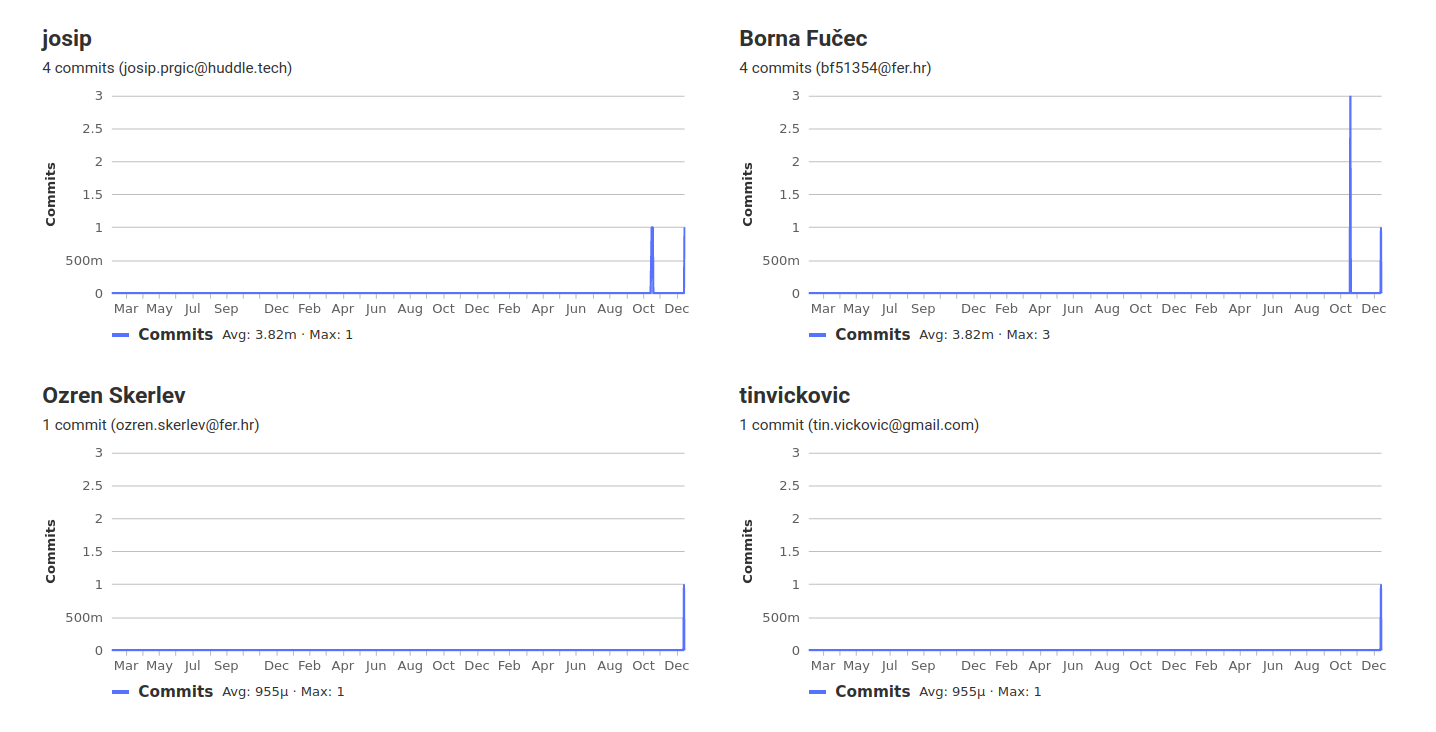
\includegraphics[scale=0.3]{slike/promjene.png}
			\centering
			\caption{Aktivnosti članova tima}
			\label{fig:promjene1}
		\end{figure}
		
	


\end{document} %naredbe i tekst nakon ove naredbe ne ulaze u izgrađen dokument 


